The studies of the \monohbb channel presented here are based on MC simulations with version 2.4.3 of \mg~\cite{Alwall:2014hca} using a Universal FeynRules Output \cite{Degrande:2011ua} implementation of the 2HDM with a Yukawa sector of type II with DM mediator~(\hdma), as provided by the authors of \cite{Bauer:2017ota}. 
The NNPDF30\_lo\_as\_0130 set of parton distribution functions (PDF) at leading order in the five-flavor scheme, which assumes a massless $b$-quark, with $\alpha_{S}(m_{Z}) = 0.130$ is used for these simulations~\cite{Ball:2014uwa}. For consistency, five-flavor scheme and $m_b=0~\GeV$ are chosen for the matrix element (ME) computation in \mg.

The ME generated for the parton-level studies presented in the following is $ g g \to h  \chi \chi$ represented in  \autoref{fig:feyn_hdm}
%ref to feynmangraph, else cite Bauer:2017ota
The only exception is the $\ma-\tanb$ scan which will be discussed in the following and is summarised in \autoref{fig:monoHbb_sensi_full_ma_tanb}. In this scan also the ME $b b \to h  \chi \chi$ is generated because at high $\tanb$, the $b b$ initiated process can have an amplitude of a similar magnitude as the gluon fusion initiated process from~\autoref{fig:feyn_hdm}~\cite{Bauer:2017ota}. 
The gluon fusion is dominant in all the remaining parameter space, therefore the $bb$ initiated process and other negligible contributions are not considered explicitly for all the scans.

\subparagraph{Signal kinematics}

The free parameters of the \hdma model fall into two categories:
\begin{itemize}
\item those which only affect total signal cross section;
\item those which, in additional to the total cross section, also affect the kinematics, primarily the \MET distribution.
\end{itemize}
In the following, the free parameters of the \hdma model are studied in the context of the \monohbb signature with a particular focus on the latter category of parameters, as it emphasizes the kinematic diversity of potential new physics contributions represented in this simplified model.


The masses $\mA$ and $\ma$ of the pseudoscalars $A$ and $a$, which represent the two mediators in \autoref{fig:feyn_hdm}, affect the kinematics of the $\monohbb$ in a profound way by changing the location of the Jacobian peak in the \MET distribution. This effect is crucial to searches for \monohbb such as  \cite{Aaboud:2017yqz}, since the $\MET$ observable can be used to reduce many SM backgrounds, which are typically characterised by low  $\MET$, unlike DM signal processes with potentially very high $\MET$. In other words, the distribution of \met determines the sensitivity of the search.

The Jacobian peak is the result of a resonantly produced pseudoscalar $A$ decaying in the $2\to1\to2$ process $gg\to A\to a h$, 
where the Higgs boson proceeds to decay into a visible final state as $h\to b b$, and the light pseudoscalar into an invisible one as $a\to \chi\chi$. 
%The kinematics of  $1\to 2$ processes are fixed by the masses of the involved particles.
Thus, the resonant $A \to a h $  process has a sharply peaked resonance in the invariant mass distribution of the final state system with a  width determined by the widths of $a$, $A$, and $h$. This results in a peak in the momentum distribution of the DM system and in its transverse component that is reconstructed as $\MET$ in the detector.
%This peak in the $\MET$ distribution resulting from the resonant signal process  is called the Jacobian peak.

Since it is determined by the masses of the particles involved in the decay, 
the location of the Jacobian peak can be calculated analytically~\cite{Bauer:2017ota}:
\begin{align}
E^{\mathrm{miss},max}_T \approx \frac{\sqrt{\left(\mA^2 -\ma^2 -M_{h}^2\right)^2 - 4 \ma^2 M_{h}^2}}{2\mA}\,.
\label{eq:monoH_peak_met}
\end{align}
Thus, increasing $\mA$ results in  a Jacobian peak at higher $\MET$, as shown in \autoref{fig:monoHbb_mA_scan_met}.
Conversely, models with higher $\ma$ have a Jacobian peak at lower $\MET$, as indicated in \autoref{fig:monoHbb_ma_scan_met}. 

\begin{figure}[tbp]
\centering
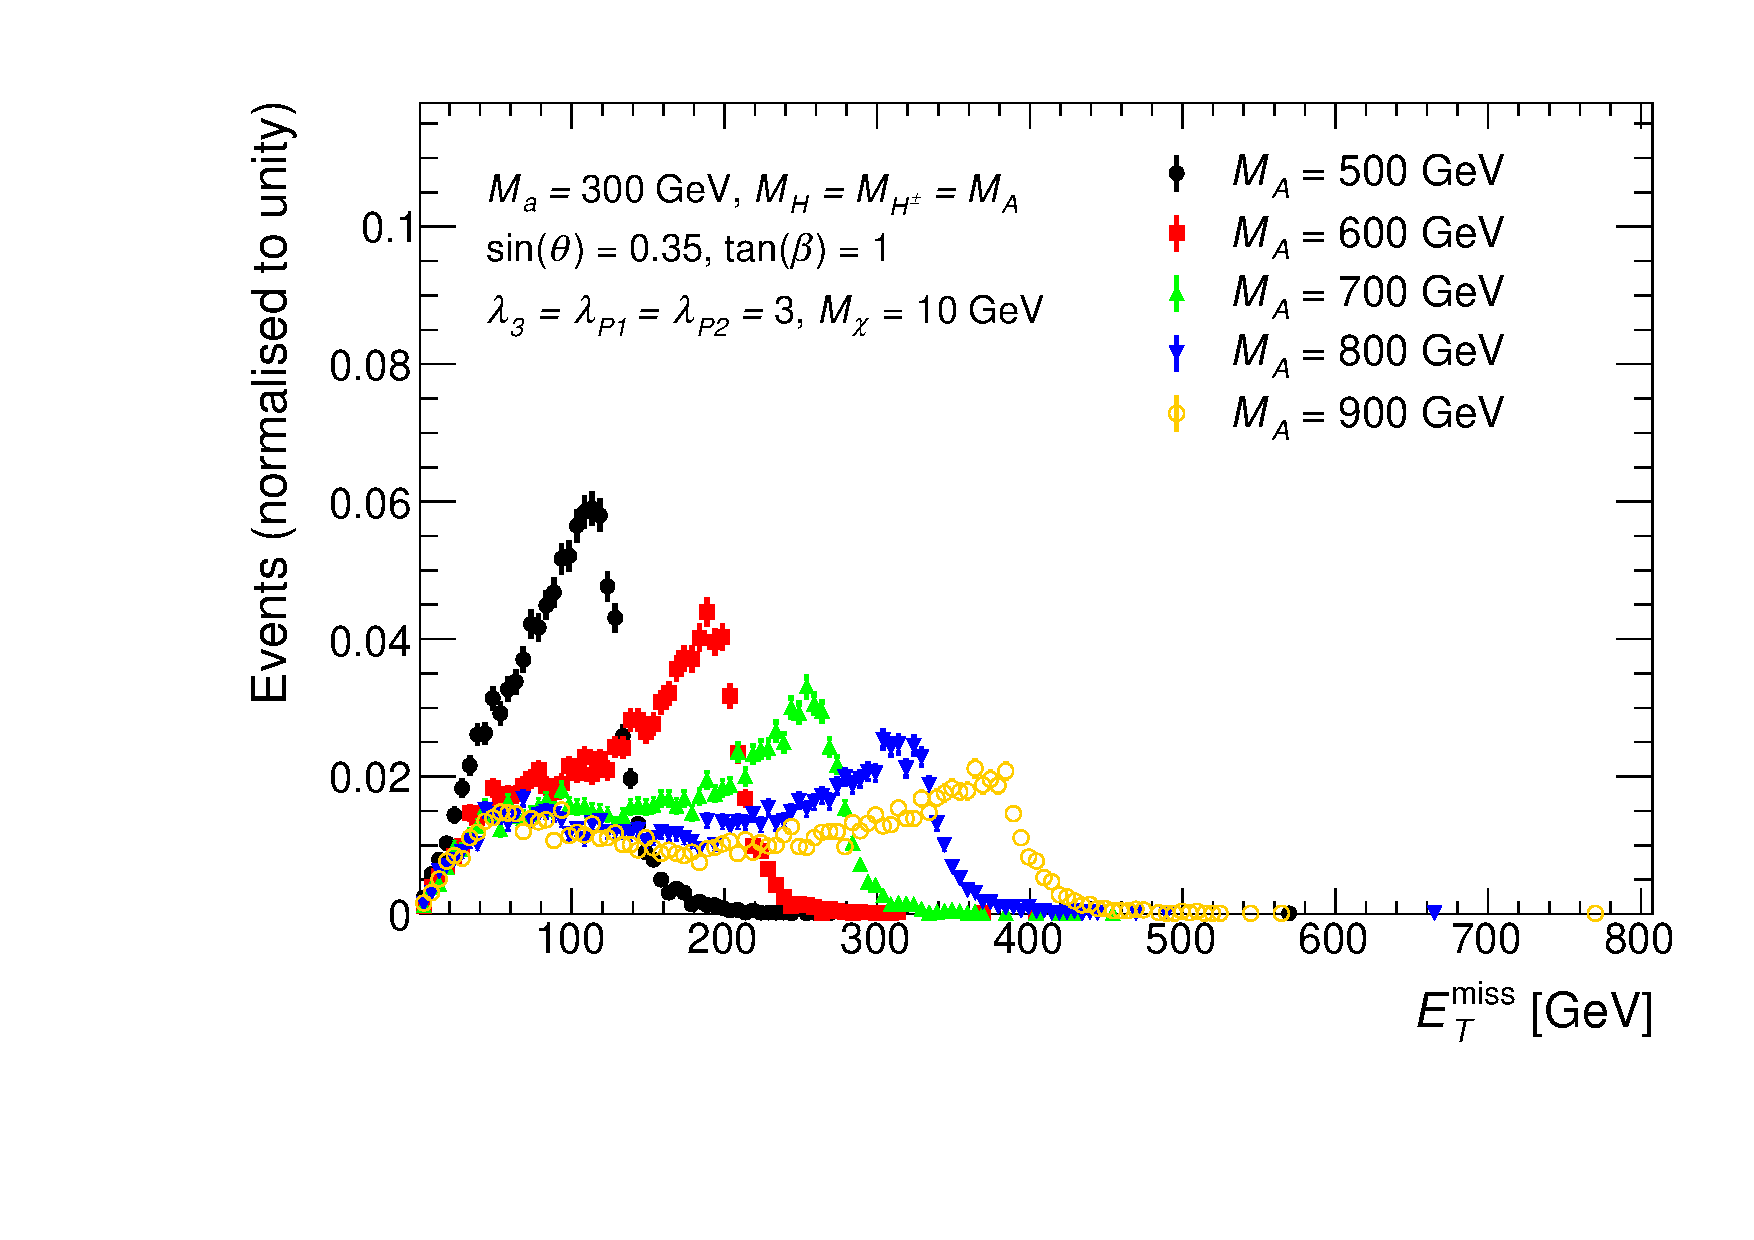
\includegraphics[width=0.7\textwidth]{texinputs/04_grid/figures/monoHbb_m_large_A_scan_MET_liny_norm2one.pdf}
\caption[$\MET$ distribution in  \monohbb events for different $\mA$]
{
Missing transverse momentum distribution  \monohbb signal events at parton level for five representative models with different $\mA(=\mH=\mHc)$
and fixed $\ma = 300$ GeV, $ \sinp = 0.35, \tanb = 1, \mDM = 10$ GeV and $ \lap1 = \lap2 = \lam3 = 3 $. 
Models with a larger $\mA-\ma$ splitting have harder \met (cf.  \autoref{eq:monoH_peak_met}). 
%
% interpretation for the text
%This is due to the resonant Jacobian peak shifting to higher values.}
}
\label{fig:monoHbb_mA_scan_met}
\end{figure}


\begin{figure}[tbp]
\centering
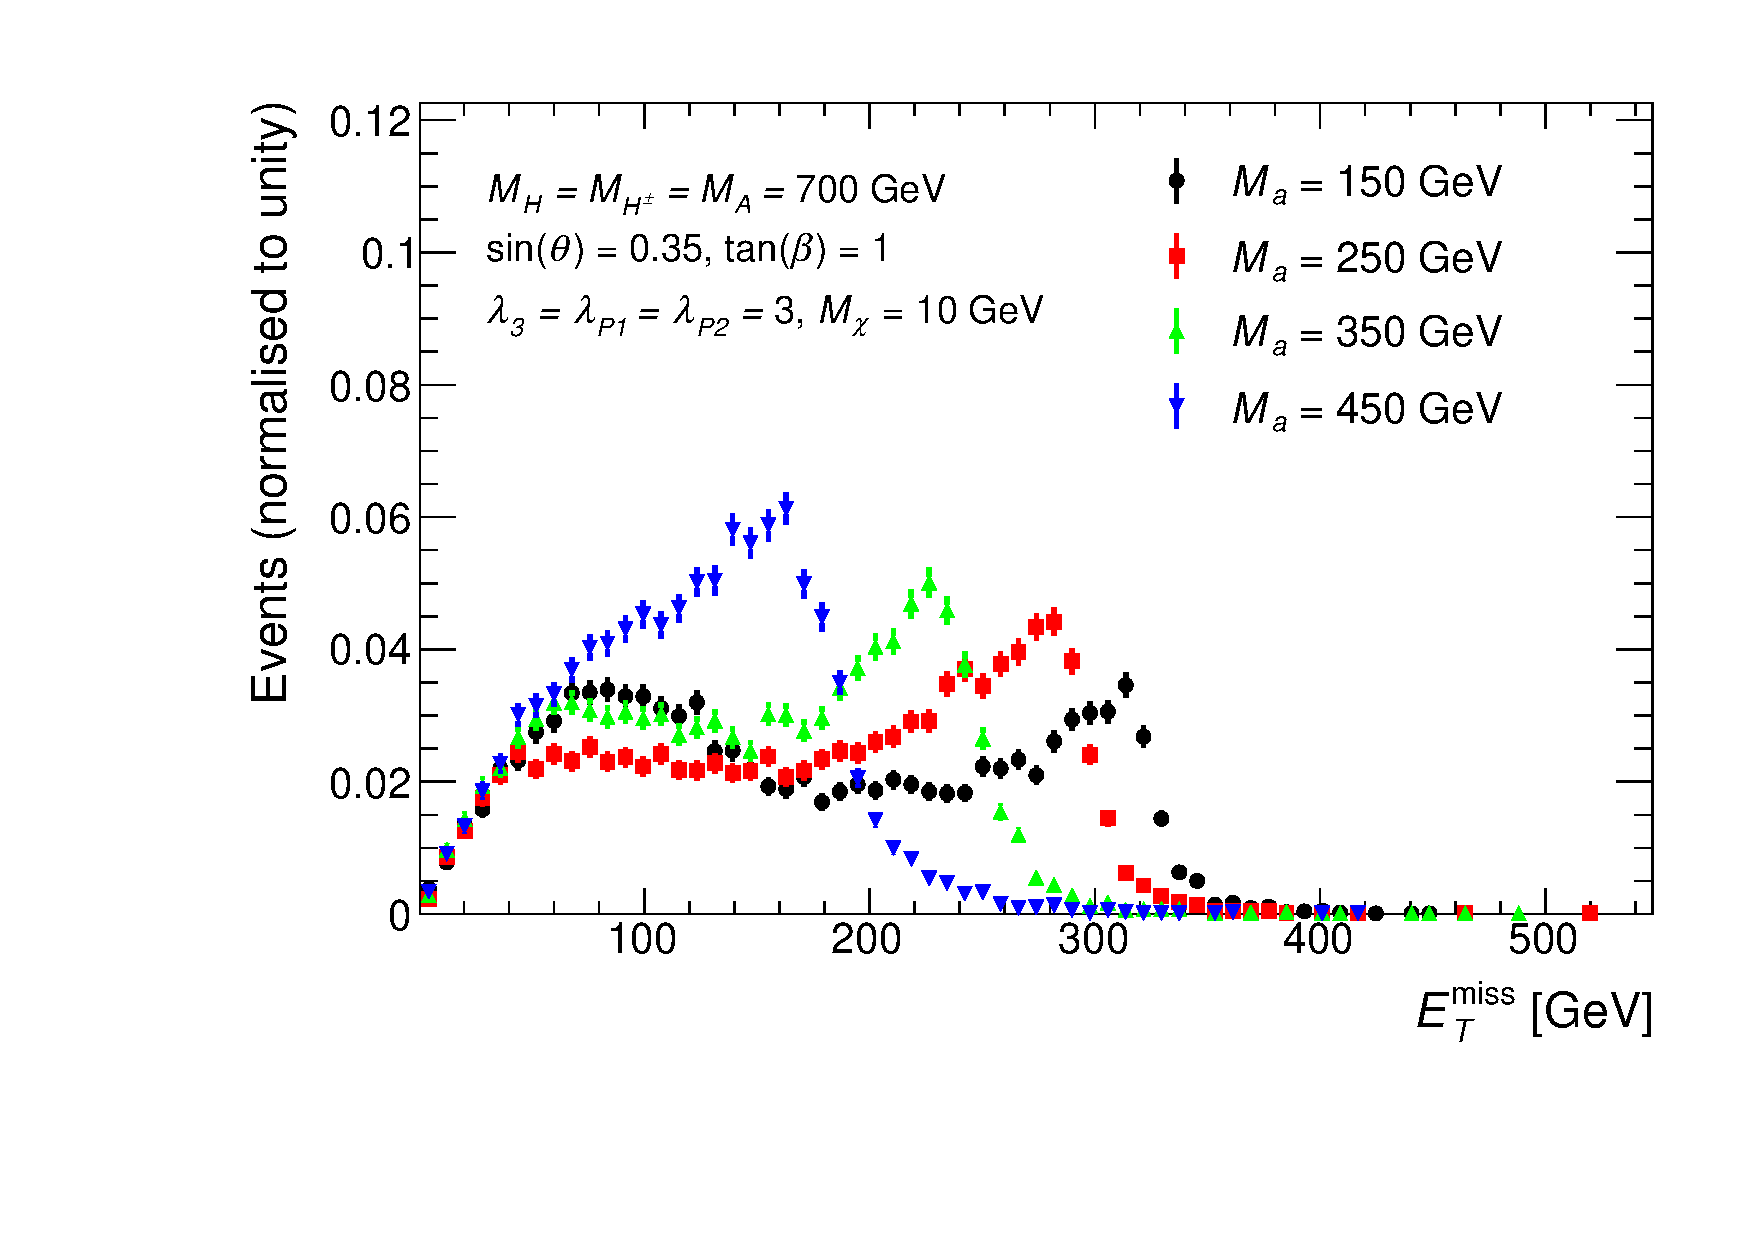
\includegraphics[width=0.7\textwidth]{texinputs/04_grid/figures/monoHbb_m_small_a_scan_MET_liny_norm2one.pdf}
\caption[$\MET$ distribution in  \monohbb events for different $\ma$]
{
Missing transverse momentum distribution in  \monohbb signal events at parton level for four representative models with different $\ma$ 
and fixed $ \mA=\mH=\mHc= 700$ GeV, $ \sinp = 0.35, \tanb = 1, \mDM = 10$ GeV and $ \lap1 = \lap2 = \lam3 = 3 $. 
Models with higher $\ma$ have softer \met (cf. \autoref{eq:monoH_peak_met}).
%
% interpretation for the text
%This is due to the resonant Jacobian peak shifting to lower values.
}
\label{fig:monoHbb_ma_scan_met}
\end{figure}


In conclusion, the $\mA$ and $\ma$ parameters strongly affect the sensitivity of a search for the \hdma model using the \monohbb signature because they determine the location of the Jacobian peak in the \met distribution. Therefore, one of the proposed parameter scans for the \hdma model is in the ($\ma$,$\mA$) plane.


Some fraction of signal events is due to non-resonant $2 \to 3$ processes $gg \to h \chi \chi$ which is represented in \autoref{fig:feyn_hdm_box}. 
%link into thereory section graph or cite paper
Due to the larger number of kinematic degrees of freedom, the  invariant mass of the final state system is broadly distributed in these processes.
Consequently, this results in a broad and soft \met distribution that is clearly distinct from the Jacobian peak discussed above.
The models shown in \autoref{fig:monoHbb_mA_scan_met} and \autoref{fig:monoHbb_ma_scan_met} also have small contributions from non-resonant processes.


The mass of the heavy neutral scalar Higgs boson $H$ has an indirect effect on the rate and kinematics of the signal. 
This is caused by the dependence of the coupling strengths and thus decay widths of  the pseudoscalars $A$ and $a$ on  $\mH$~\cite{Bauer:2017ota}. 
Therefore, a change of $\mH$ can affect the relative contribution of resonant versus non-resonant signal processes, as illustrated in \autoref{fig:monoHbb_mH_scan_met}.  
The choice $\mH = \mA$ results in a detectable total cross section for many signal points and a dominant contribution of the resonant signal process, resulting in diverse experimental signatures as demonstrated in \autoref{fig:monoHbb_mA_scan_met} and \autoref{fig:monoHbb_ma_scan_met}. In addition, this choice results in about equal contributions to the sensitivity through the \monoz and \monoh signatures, highlighting their complementarity. Henceforth,  $\mH = \mA$ is adapted for all scans. For simplicity, the case of the neutral scalar $H^{\pm}$ being mass-degenerate to $H$ is considered in the following, as it does not affect the \hdma model kinematics in the \monohbb signature.

\begin{figure}[tbp]
\centering
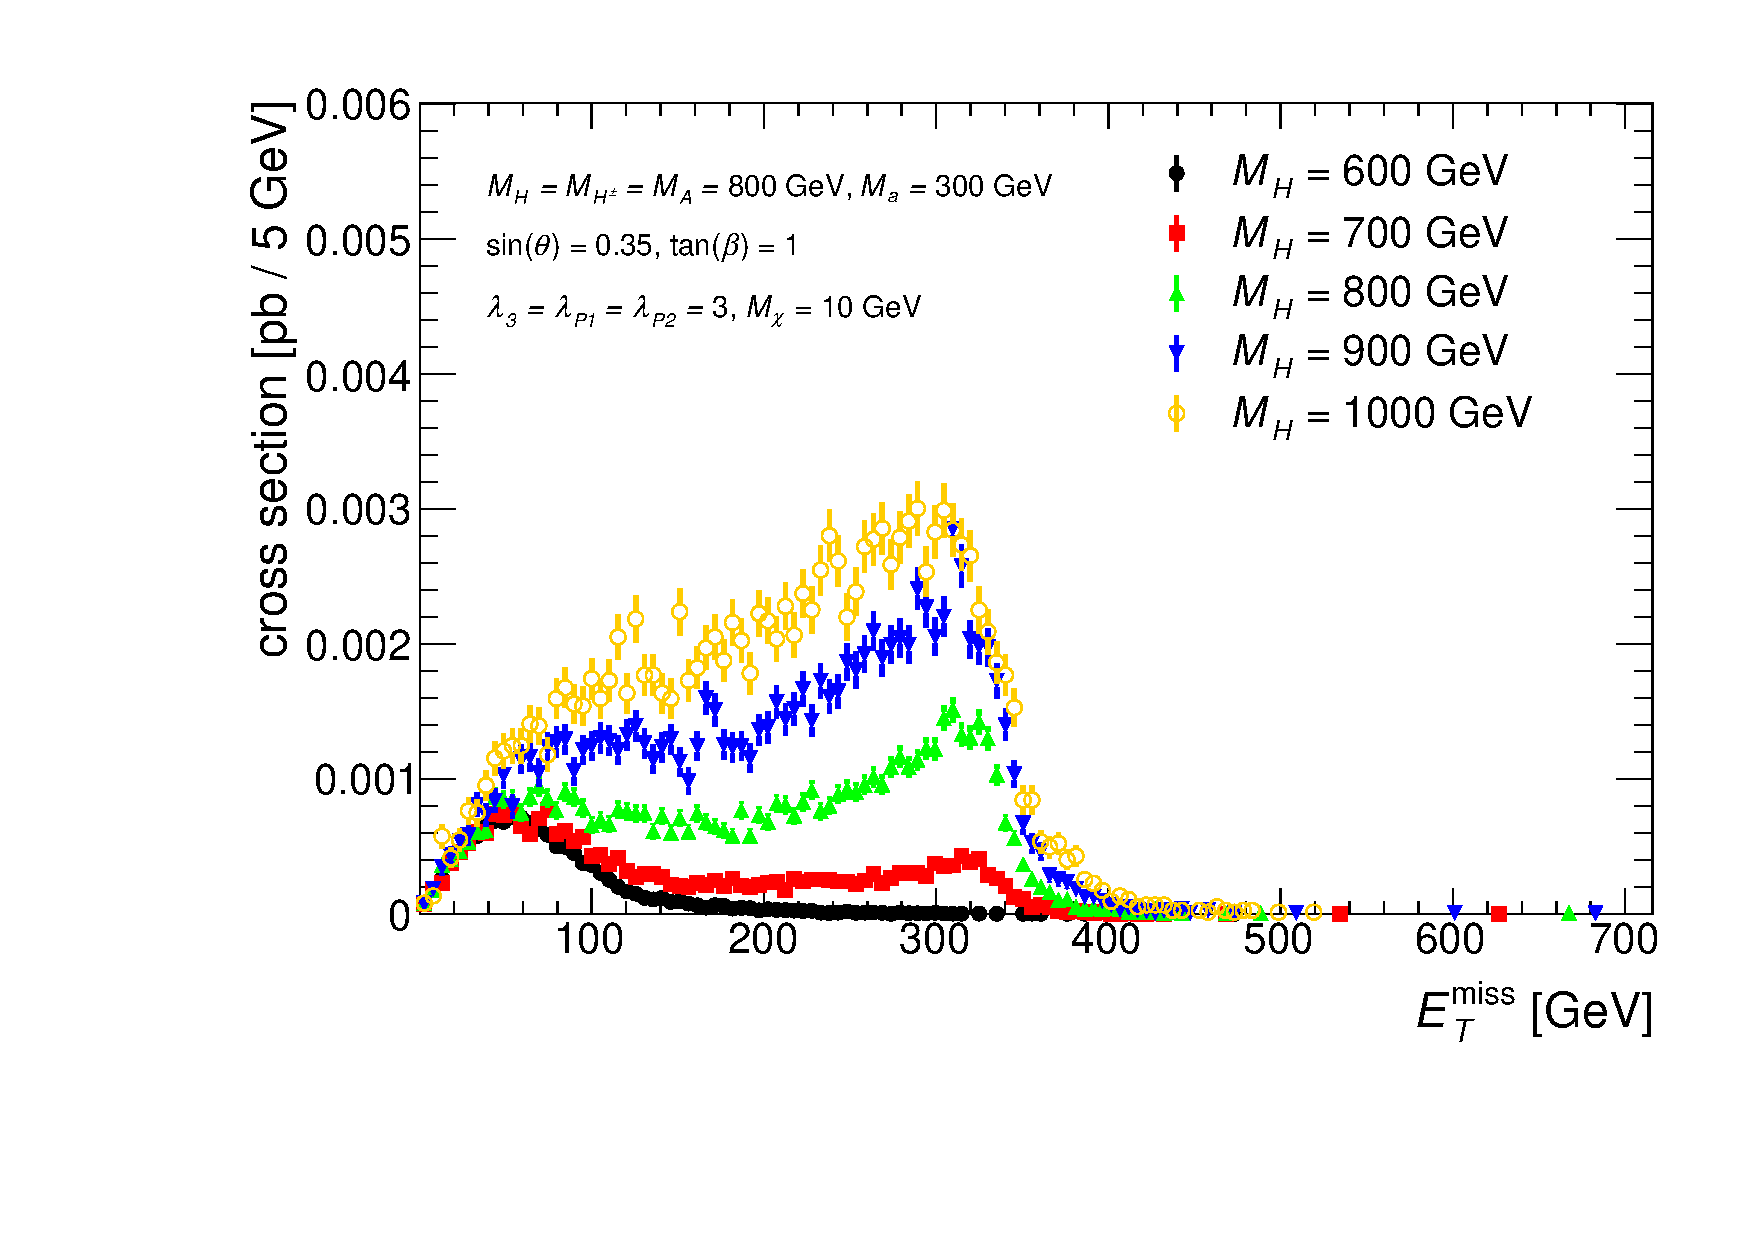
\includegraphics[width=0.7\textwidth]{texinputs/04_grid/figures/monoHbb_mH_scan_MET_liny.pdf}
\caption[$\MET$ distribution in \monohbb events for different $\mH$]
{The \MET distribution of the production cross section of \monohbb signal events for five representative models with different $\mH = \mHc$ 
and fixed $ \mA=800$ GeV, $\ma = 300 $ GeV,  $ \sinp = 0.35, \tanb = 1, \mDM = 10$ GeV and $ \lap1 = \lap2 = \lam3 = 3 $. 
%
% interpretation for the text
%Models with $\mH = \mHc \geq \mA $ have a stronger resonant contribution, and a larger cross section. The resonant contribution is enhanced more strongly with higher $\mH = \mHc$. For $\mH = \mHc < \mA$ the resonant contribution is suppressed.
}
\label{fig:monoHbb_mH_scan_met}
\end{figure}



%%%%% text related to scan of sinp
The sine of the mixing angle between the two pseudoscalars $A$ and $a$, $\sinp$,
affects not only the cross section, but also the shape of the \MET\ distribution, as shown in \autoref{fig:monoHbb_sinp_scan_mA600_ma200_met}. 
For the resonant diagram $gg\rightarrow A \rightarrow ah \rightarrow \chi\bar{\chi}h$, 
the product of cross section times branching ratios 
${\cal B}(A\rightarrow ah){\cal B}(a \rightarrow \chi\bar{\chi})$ 
scales with $\sin^2\theta\cos^6\theta$, while for the diagram 
$gg\rightarrow a \rightarrow A^*h \rightarrow \chi\bar{\chi}h$, the 
product of cross section times branching ratios 
${\cal B}(a\rightarrow Ah){\cal B}(A \rightarrow \chi\bar{\chi})$ 
scales with $\sin^6\theta\cos^2\theta$. Therefore, at small \sinp, the resonant 
diagram $A\rightarrow ah$ is the dominant production mode and the \MET\ distribution 
has a Jacobian peak following \autoref{eq:monoH_peak_met}; while at large \sinp, the 
$a\rightarrow A^*h$ diagram starts to dominate and produces a second peak at a lower 
\MET\ value.


\begin{figure}[tbp]
\centering
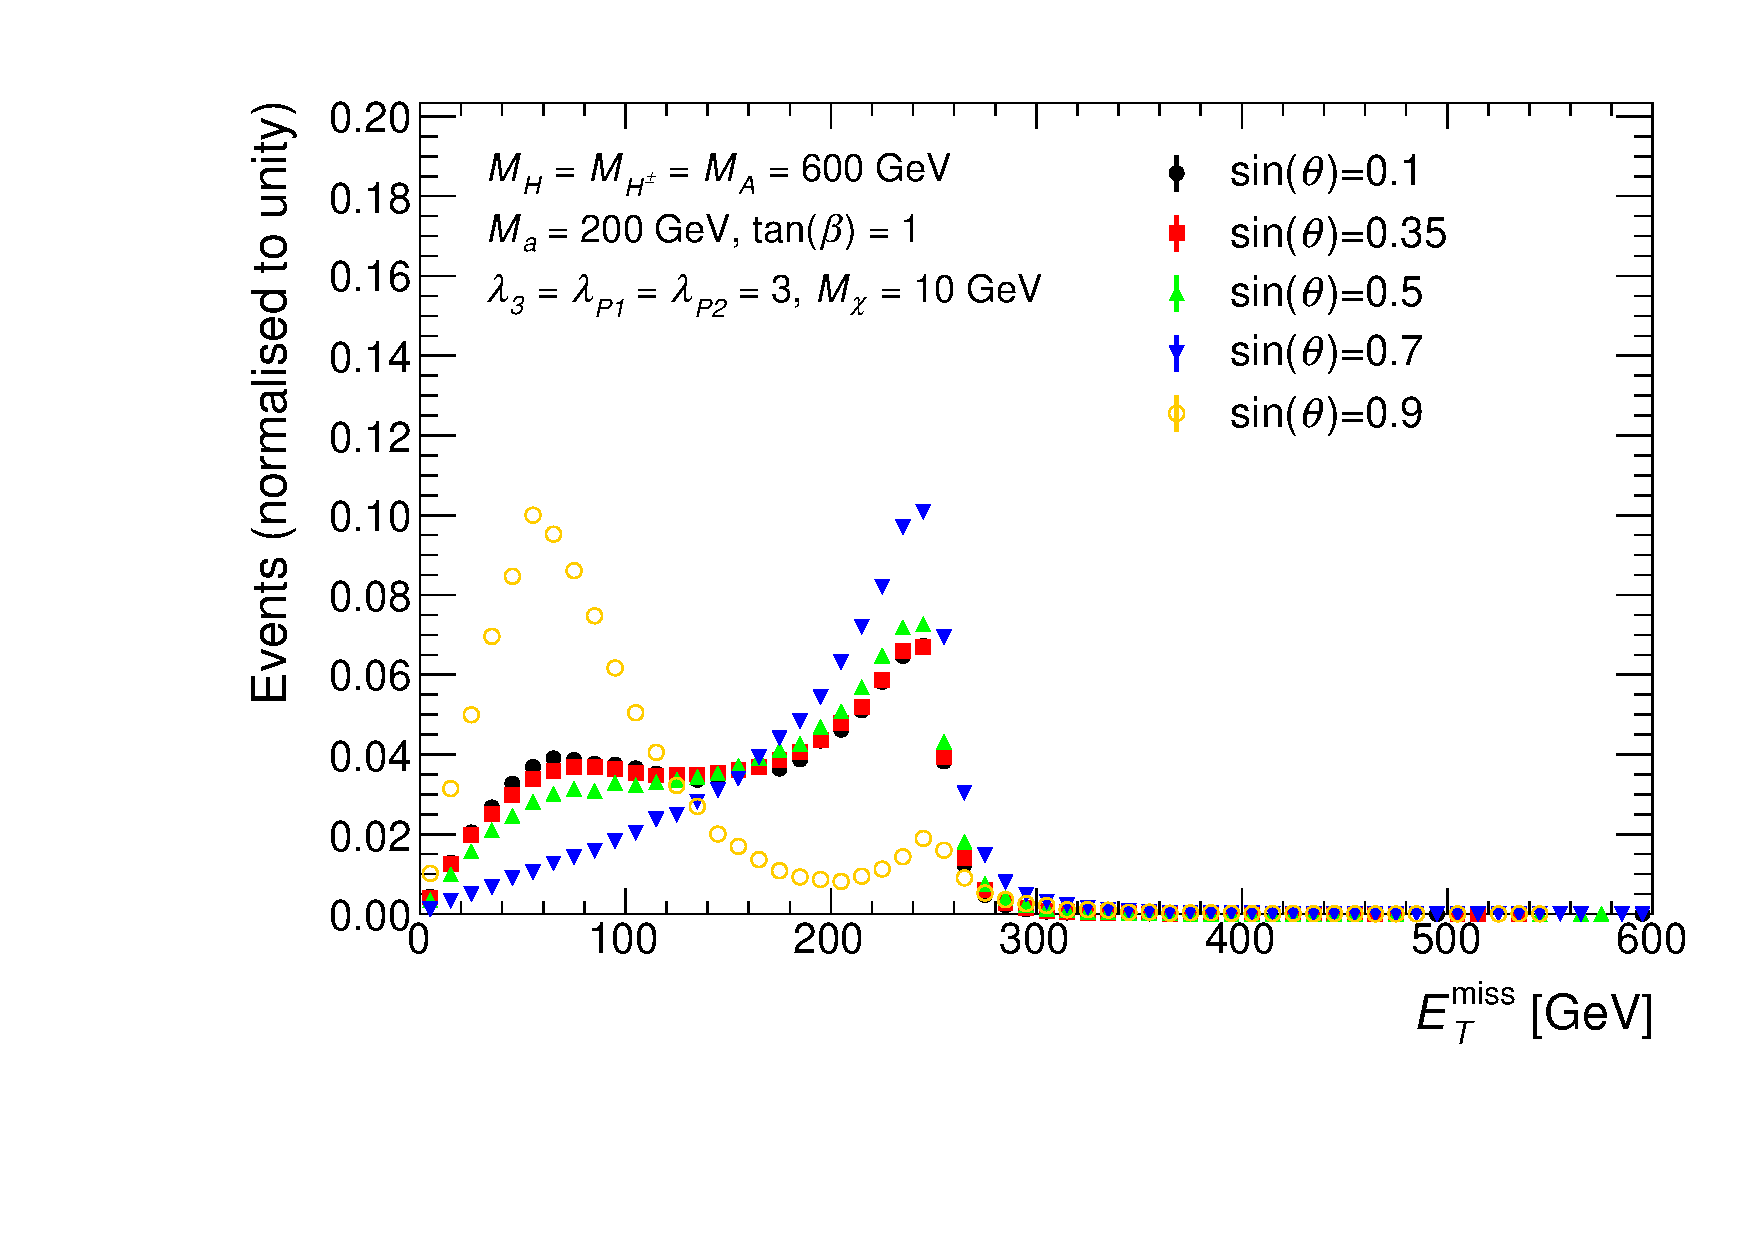
\includegraphics[width=0.7\textwidth]{texinputs/04_grid/figures/monoHbb_sinp_scan_MA600_Ma200_MET_liny_norm2one.pdf}
\caption[$\MET$ distribution in $h\rightarrow bb + \MET$ events for different 
$\sinp$ for $\mA = \mH = \mHc = 600 $ GeV and $\ma = 200$ GeV]
{
Missing transverse momentum distribution of $h\rightarrow bb + \MET$ signal 
events at parton level for five representative models with different $\sinp$ and
 fixed $\mA = \mH = \mHc = 600 $~GeV, $\ma = 200$~GeV, $ \mDM = 10$~GeV, $\tanb = 1$, 
and $ \lap1 = \lap2 = \lam3 = 3 $. 
The shape of the $\MET$ distribution does not change much  
for $\sinp < 0.7$, then changes significantly for $\sinp\geq 0.7$. 
When $\sinp=0.9$, the diagram $gg\rightarrow a\rightarrow A^*h \rightarrow \chi \bar{\chi} h$, 
producing a \MET peak at around 60~GeV, starts to dominate.
%
}
\label{fig:monoHbb_sinp_scan_mA600_ma200_met}
\end{figure}



%%% text related to tanbeta-ma scan
The shape of \MET\ distribution also has a non-trivial dependence on \tanb, as can be seen in \autoref{fig:monoHbb_tanb_scan_met}.
As discussed in the sensitivity study later, at small \tanb, the Yukawa coupling 
to top quark is large and the signal production mode is dominated by the 
non-resonant 3-body processes $gg\rightarrow h\chi\bar{\chi}$, which gives a broad 
and soft \MET\ spectrum. As \tanb increases, the contribution of 
resonant production increases as well and the Jacobian peak also appears.
When the pseudoscalar $A$ is produced off-shell, i.e. when $\mA<\ma+\mh$, the shapes 
of \MET\ distributions become similar and the dependence on \tanb disappears.


\begin{figure}[tbp]
\centering
\begin{subfigure}{0.48\textwidth}
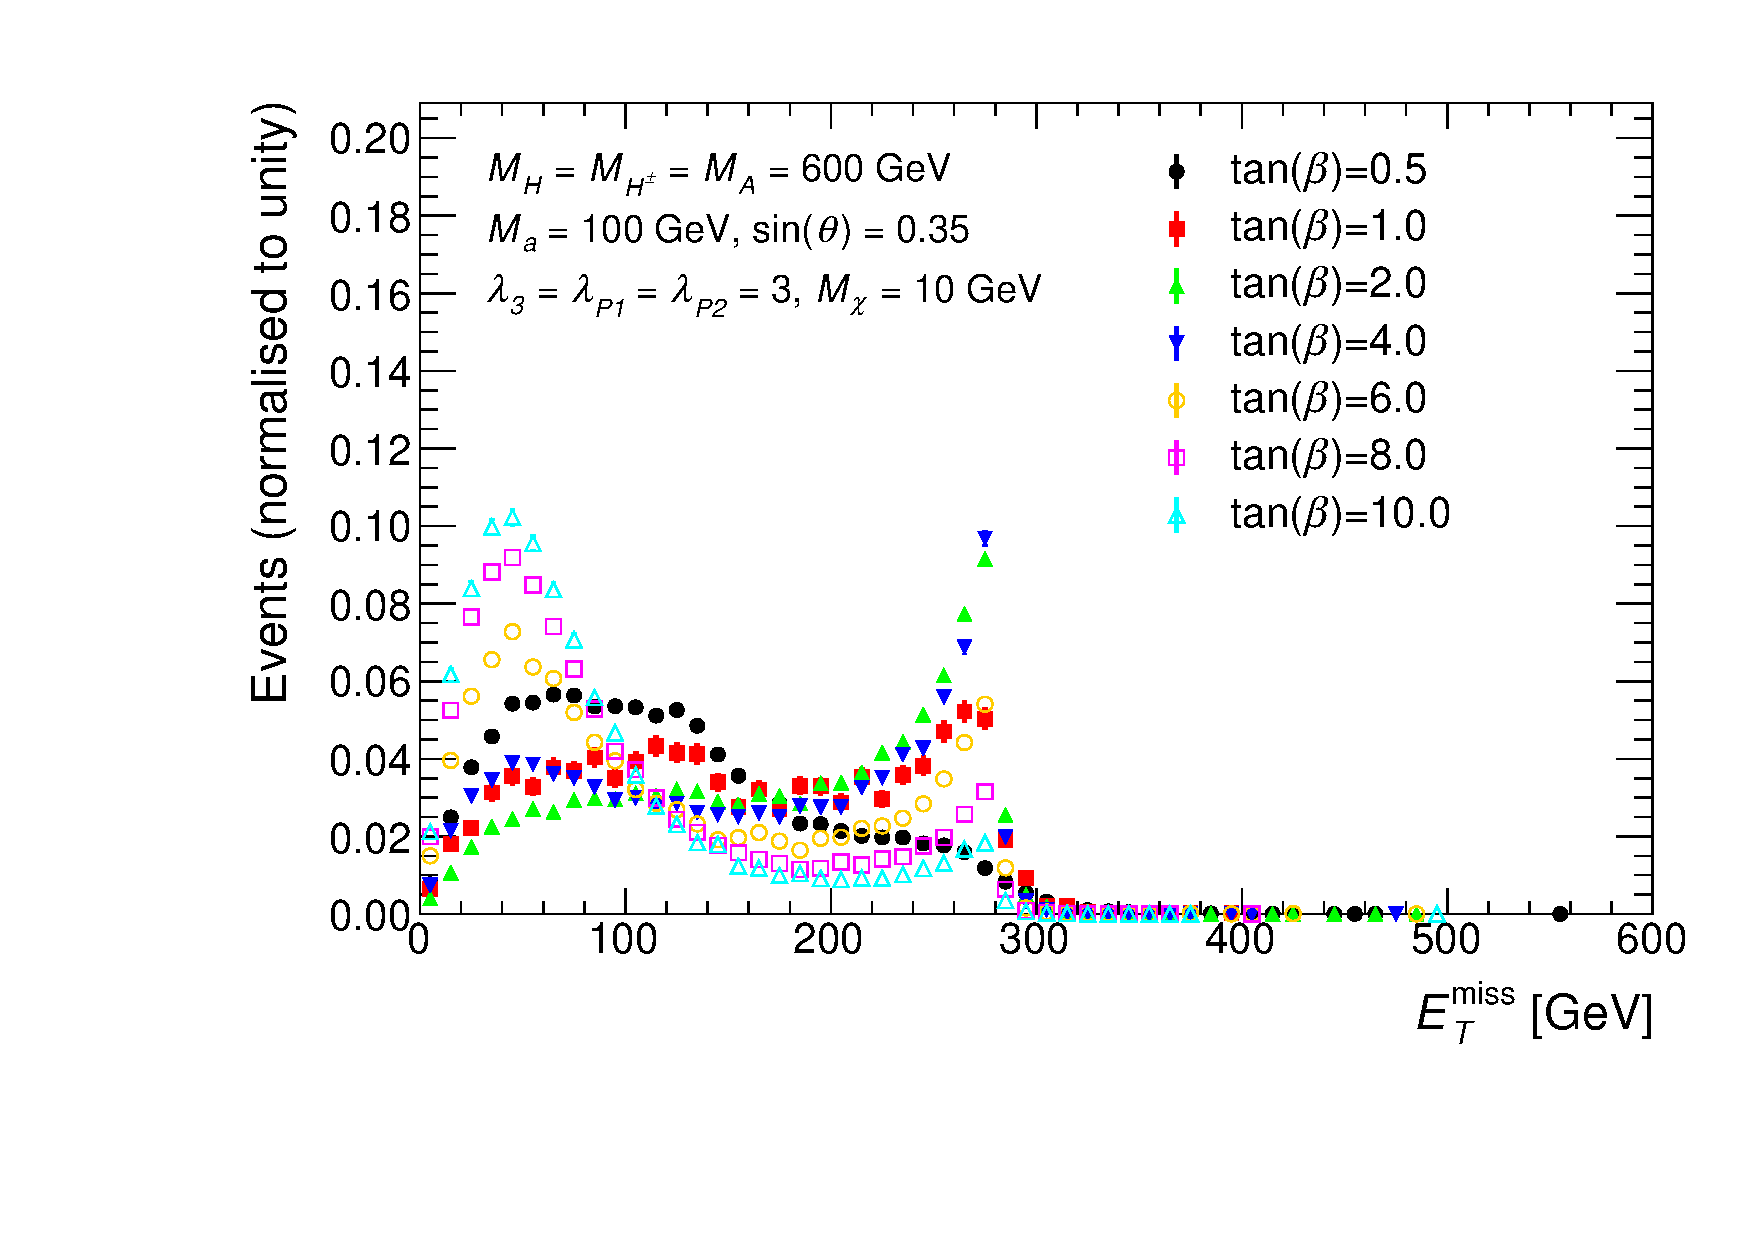
\includegraphics[width = \textwidth]{texinputs/04_grid/figures/monoHbb_tanb_scan_MA600_Ma100_MET_liny_norm2one.pdf}
\end{subfigure}
~
\begin{subfigure}{0.48\textwidth}
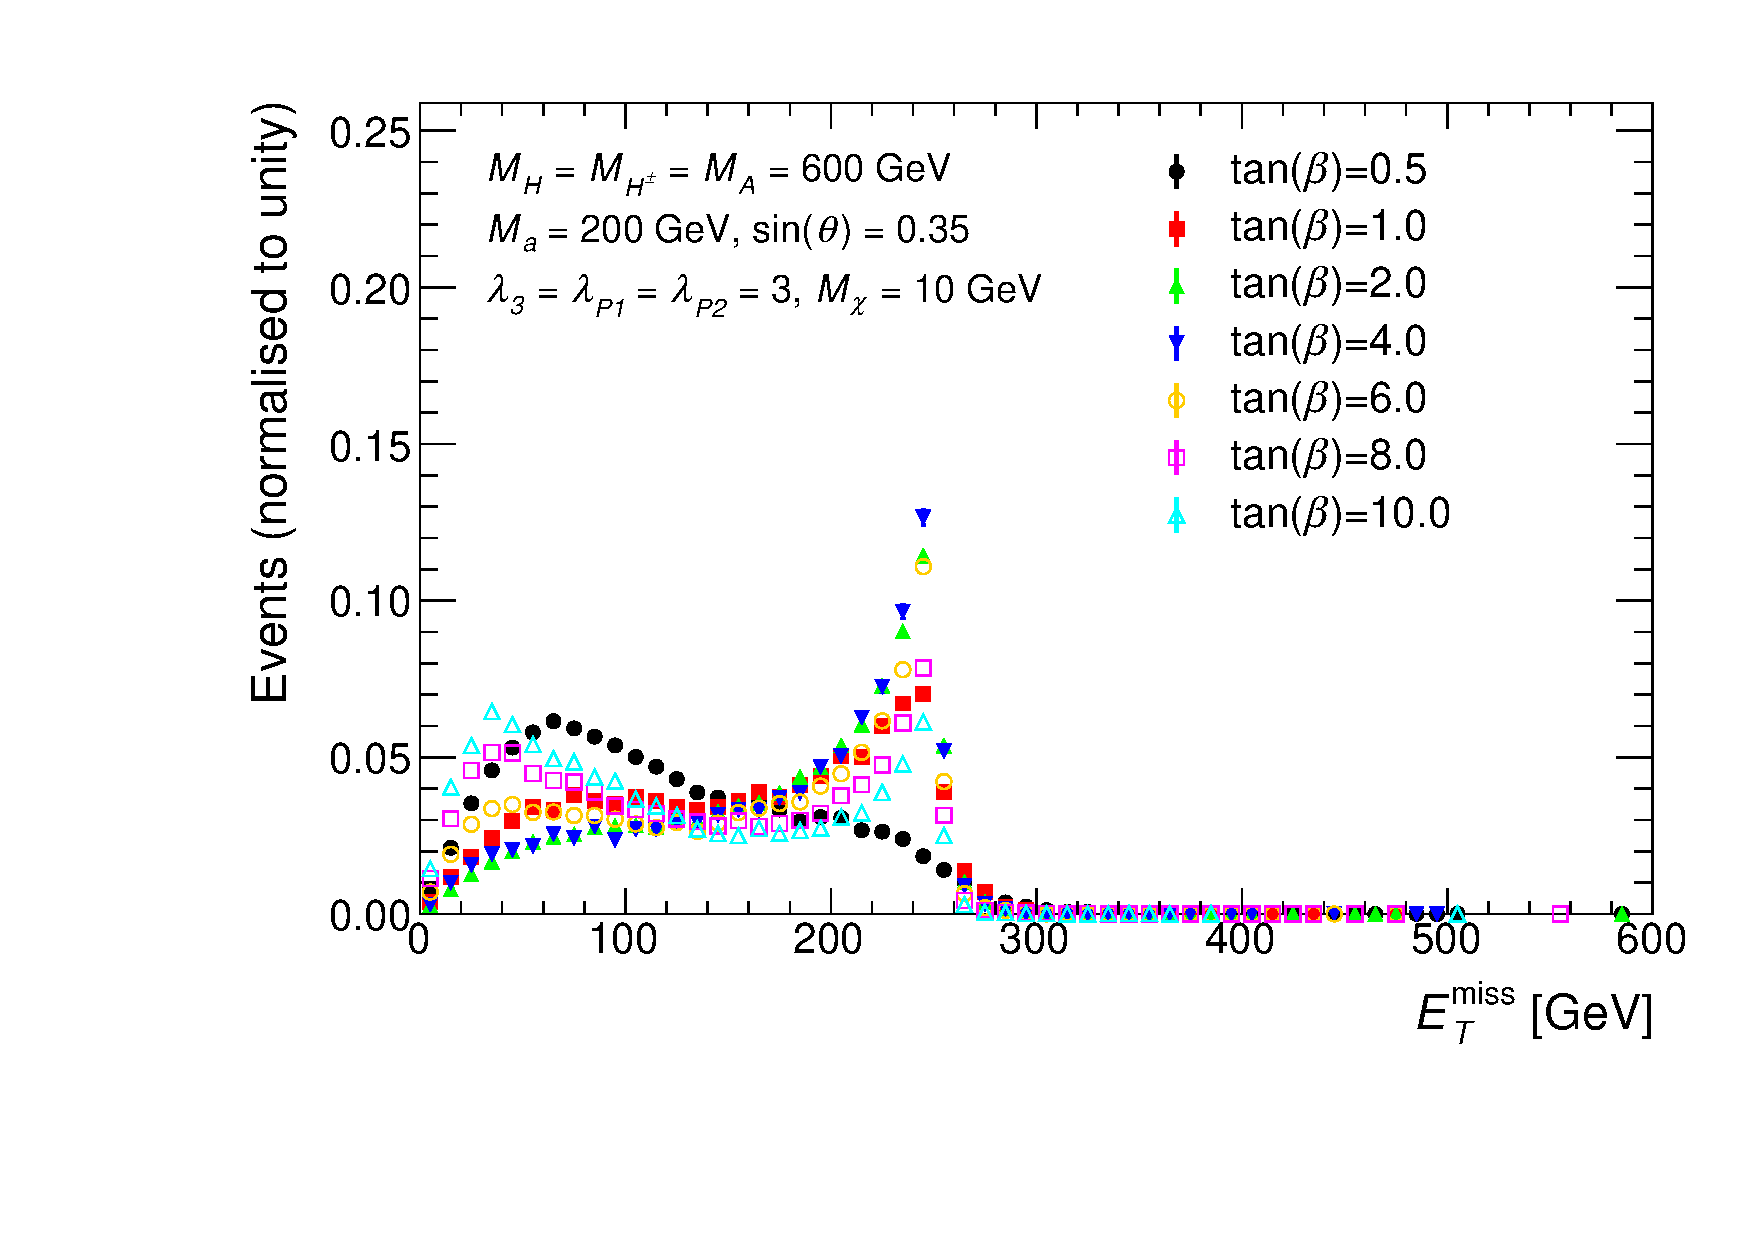
\includegraphics[width = \textwidth]{texinputs/04_grid/figures/monoHbb_tanb_scan_MA600_Ma200_MET_liny_norm2one.pdf}
\end{subfigure}
\\
\centering
\begin{subfigure}{0.48\textwidth}
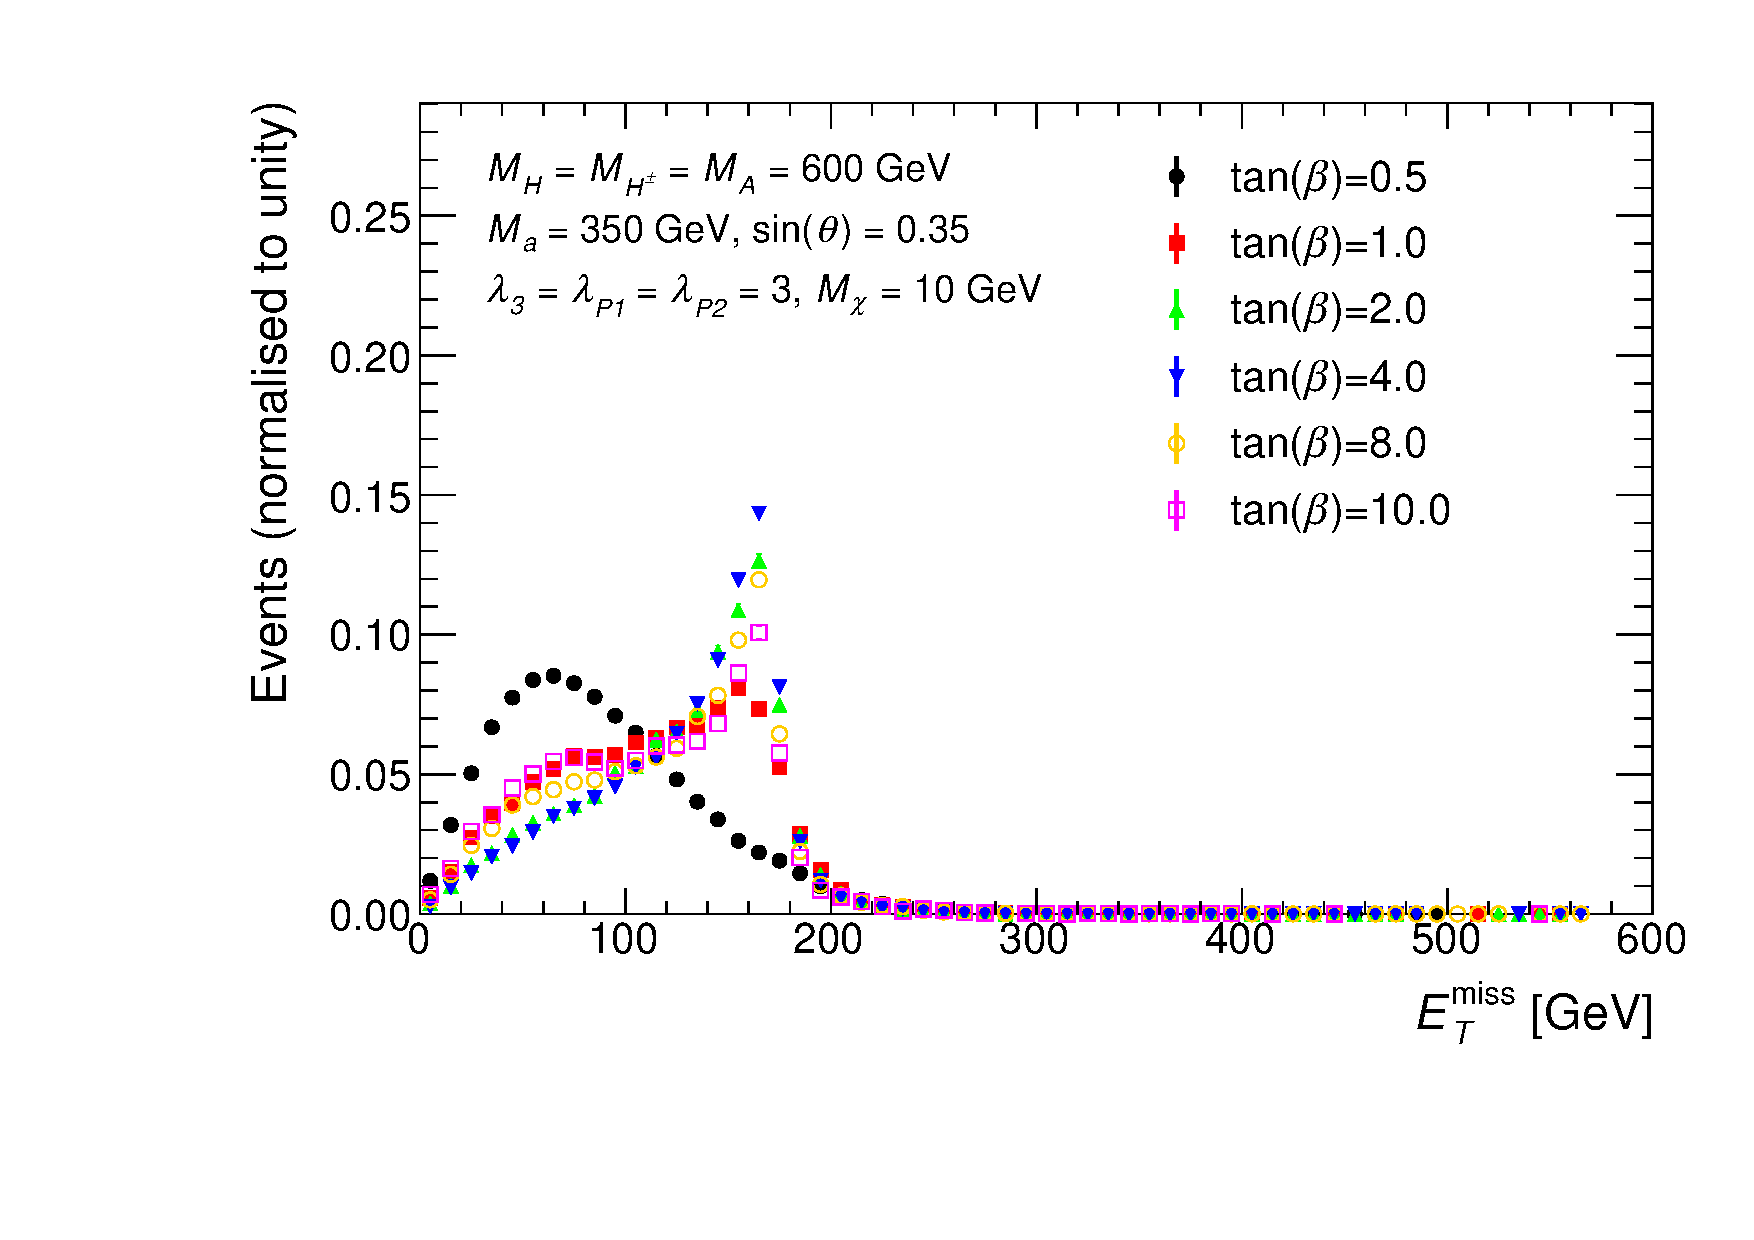
\includegraphics[width = \textwidth]{texinputs/04_grid/figures/monoHbb_tanb_scan_MA600_Ma350_MET_liny_norm2one.pdf}
\end{subfigure}
~
\begin{subfigure}{0.48\textwidth}
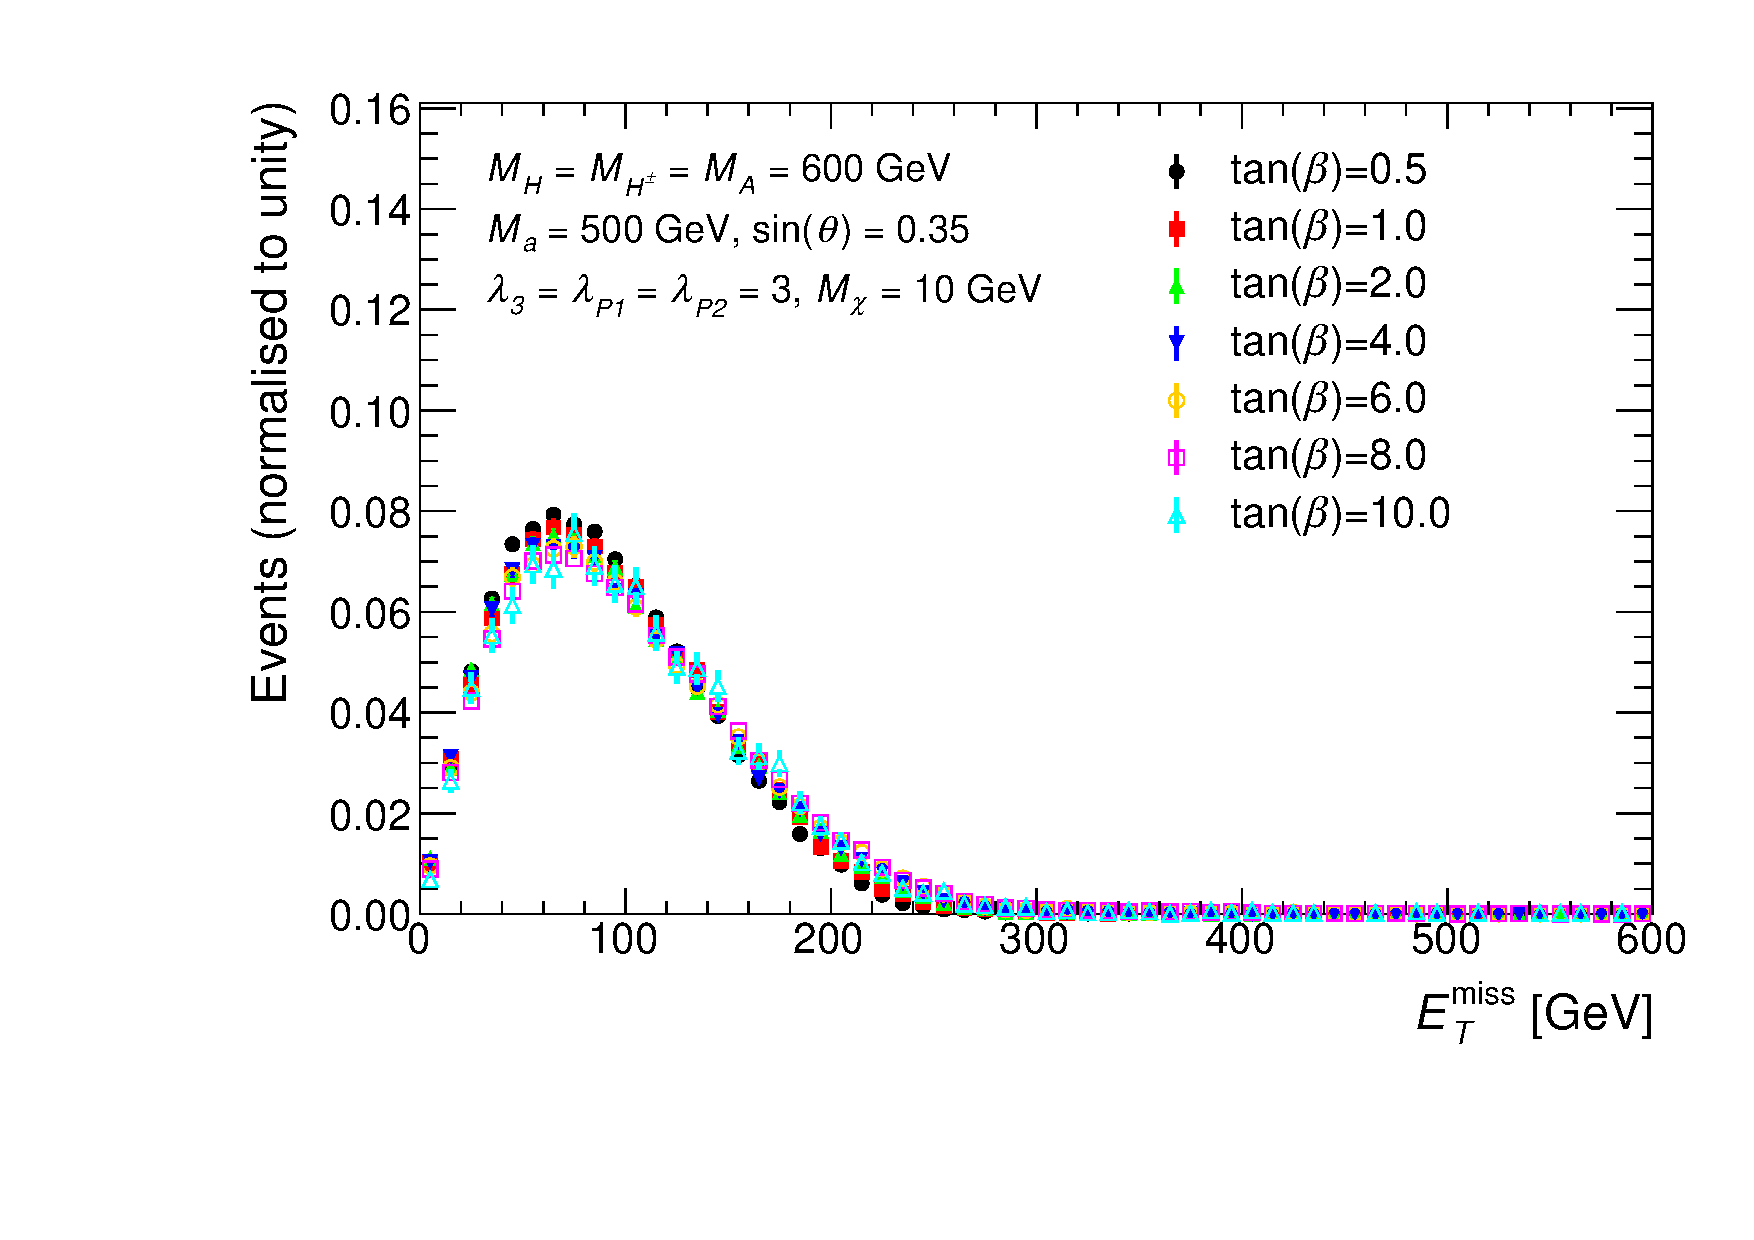
\includegraphics[width = \textwidth]{texinputs/04_grid/figures/monoHbb_tanb_scan_MA600_Ma500_MET_liny_norm2one.pdf}
\end{subfigure}
\caption[$\MET$ distribution in $h\rightarrow bb + \MET$ events for different 
$\tanb$ for $\mA = \mH = \mHc = 600 $ GeV]
{
Missing transverse momentum distribution of $h\rightarrow bb + \MET$ signal 
events at parton level with different $\tanb$ and
 fixed $\mA = \mH = \mHc = 600 $~GeV, $ \mDM = 10$~GeV, $\sinp = 0.35$, 
and $ \lap1 = \lap2 = \lam3 = 3 $. The values of $\ma$ are set to 100, 200, 
350, and 500~GeV, respectively.
The shapes of the $\MET$ distributions for different $\tanb$ are similar when 
$\mA < \mh+\ma$. Note, in these figures, both the contributions of $gg$ and $b\bar{b}$ 
initiated processes are included and a combined histogram is produced 
according to their corresponding cross sections.
}
\label{fig:monoHbb_tanb_scan_met}
\end{figure}



%\textcolor{red}{[CMS contribution]}
%The $\lambda$ parameters ...

The mass of the DM fermion $\mDM$ can change the total cross section and shape of the $\MET$ distribution,
depending on the mass hierarchy of the $A,a,h,\chi$ particles. This is demonstrated in \autoref{fig:monoHbb_mDM_scan_met}. 
Provided on-shell  decays $a\to\chi\chi$ are possible, i.e., $\mDM < \ma/2$, the exact value of \mDM has no effect on either kinematics or the total cross section. 
The only exception is the case $\ma/2 > \mDM > \frac{1}{2}(\ma - M_h)$. In this  $\mDM$ range, the non-resonant process $a \to h A^*\left(\chi\chi\right) $ is kinematically inaccessible. 
This reduces the overall cross section relative to the $\mDM \leq \frac{1}{2}(\ma - M_h)$ case, and slightly changes the soft part of the total $\MET$ spectrum. 
But since the contribution of the $a \to h A^*\left(\chi \chi\right)$ is minor in any case, the differences are negligible.

If the DM particle mass is exactly on threshold, i.e., $\mDM = \ma/2$, the total cross section is resonantly enhanced. 
This resonant threshold enhancement drops rapidly towards both higher and lower $\mDM$. Furthermore, the shape of the $\MET$ distribution at threshold, 
where amplitudes involving $a\to\chi\chi$ decays make up a larger fraction of the signal, differs significantly from the one below threshold. Below threshold ($\mDM > \ma/2$), the total cross section quickly drops by several orders of magnitude. In this regime, 
the shape of the $\MET$ distribution changes with $\mDM$ continuously.

\begin{figure}[tbp]
\centering
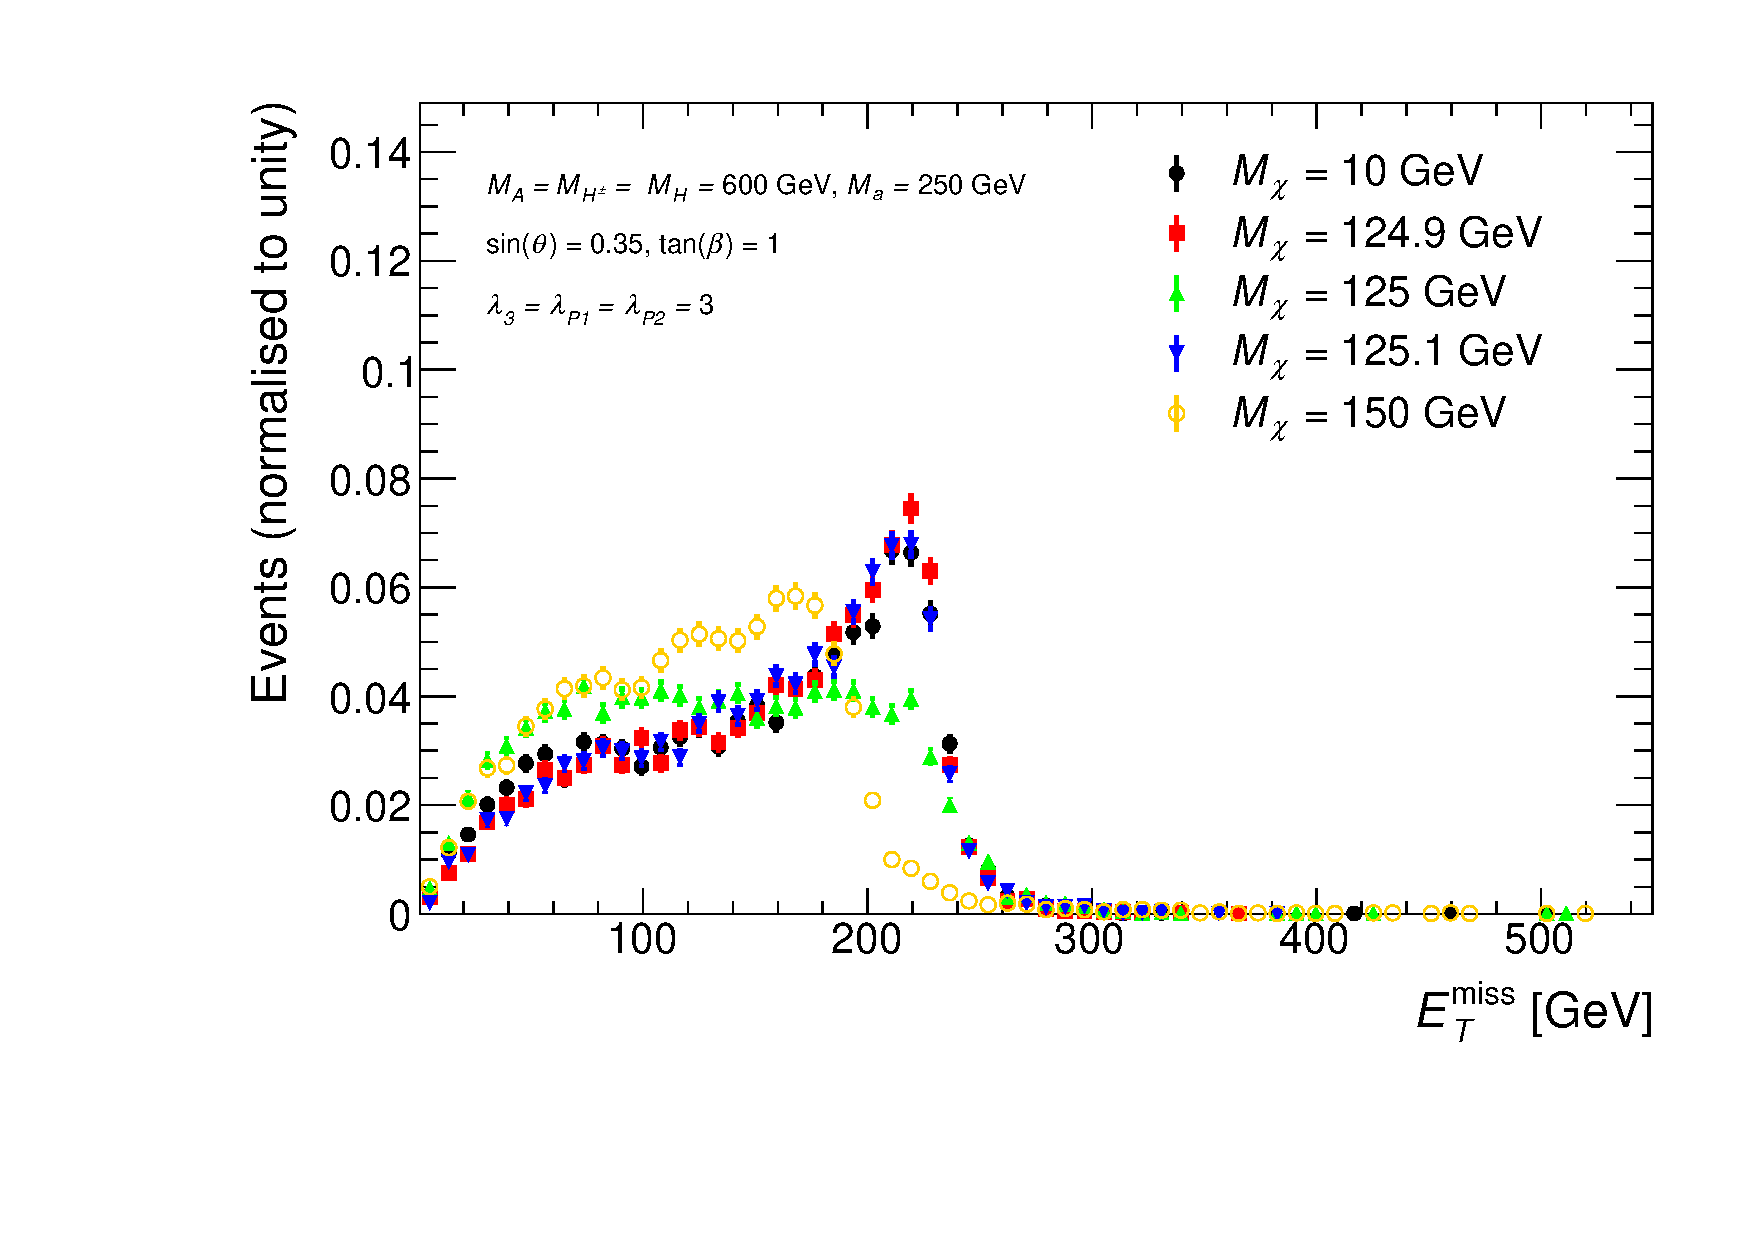
\includegraphics[width=0.7\textwidth]{texinputs/04_grid/figures/monoHbb_mDM_scan_MET_liny_norm2one.pdf}
\caption[$\MET$ distribution in \monohbb events for different $\mDM$]
{
Missing transverse momentum distribution  of \monohbb signal events at parton level for five representative models with different $\mDM$
and fixed $\mA = \mH = \mHc = 600 $ GeV $\ma = 250$ GeV, $ \sinp = 0.35, \tanb = 1$ and $ \lap1 = \lap2 = \lam3 = 3 $. 
The shape of the $\MET$ distribution does not change for $\mDM < \ma/2$, then changes significantly for $\mDM>=\ma/2$.
%
}
\label{fig:monoHbb_mDM_scan_met}
\end{figure}



\subparagraph{Sensitivity estimate}
\begin{figure}[tbp]
\centering
\begin{subfigure}{0.48\textwidth}
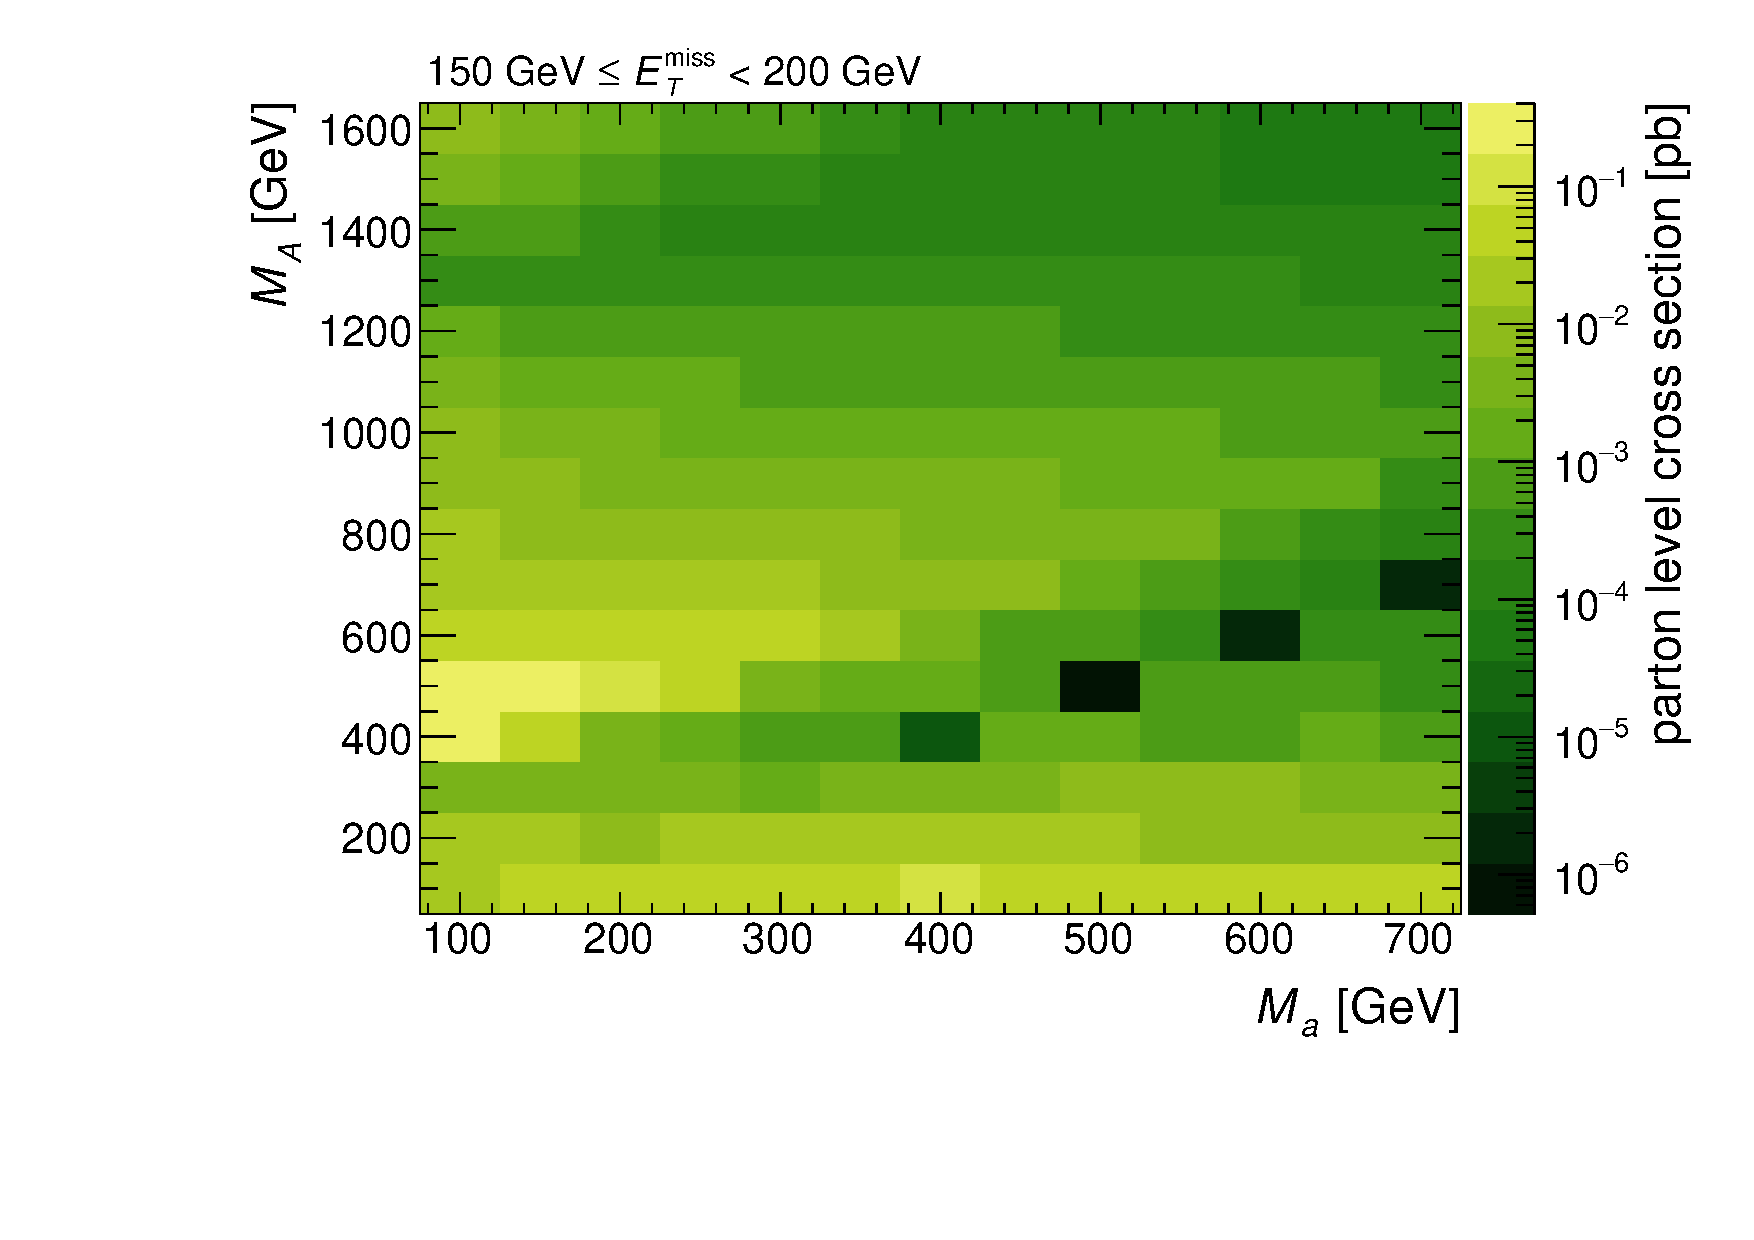
\includegraphics[width = \textwidth]{texinputs/04_grid/figures/monoHbb_parton_level_cross_section_bin_1_ma_vs_mA_lin.pdf}
\end{subfigure}
~
\begin{subfigure}{0.48\textwidth}
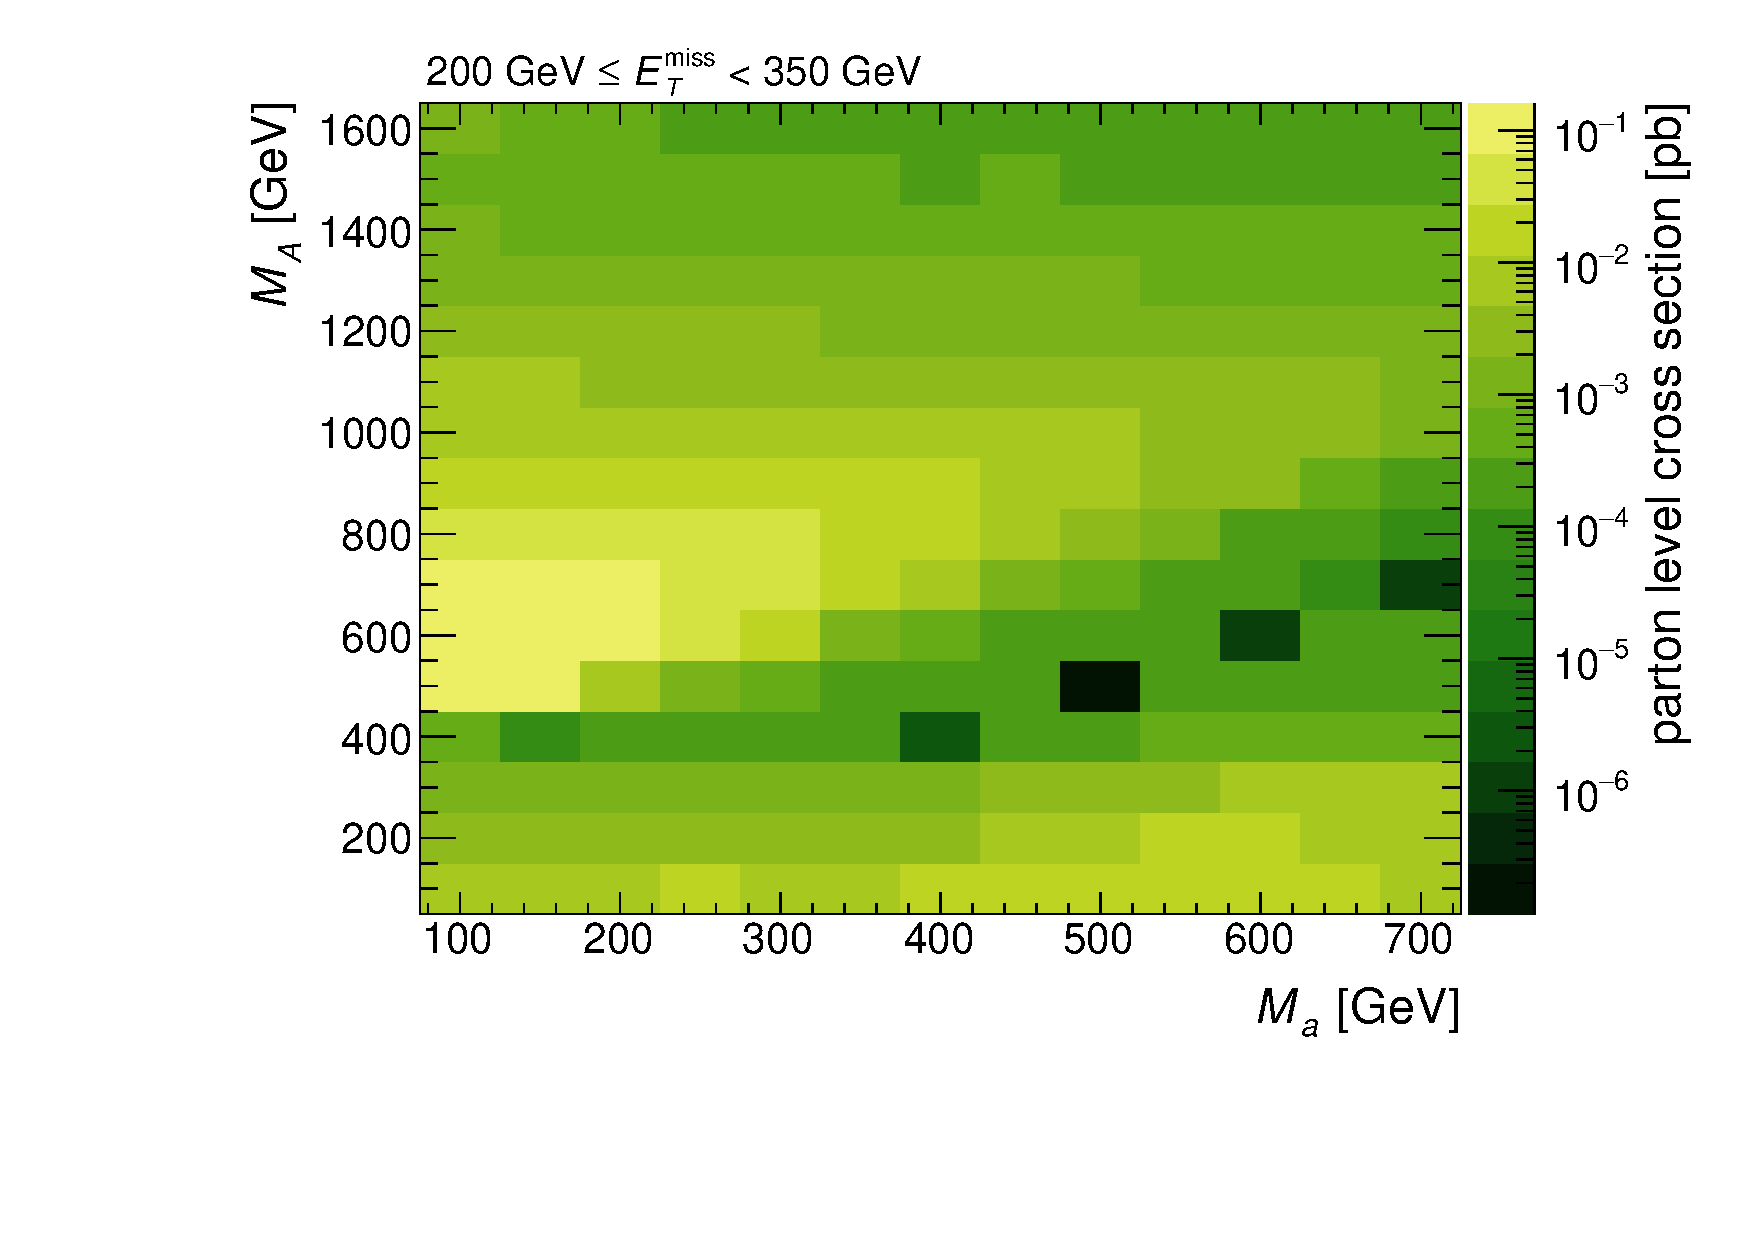
\includegraphics[width = \textwidth]{texinputs/04_grid/figures/monoHbb_parton_level_cross_section_bin_2_ma_vs_mA_lin.pdf}
\end{subfigure}
\\
\centering
\begin{subfigure}{0.48\textwidth}
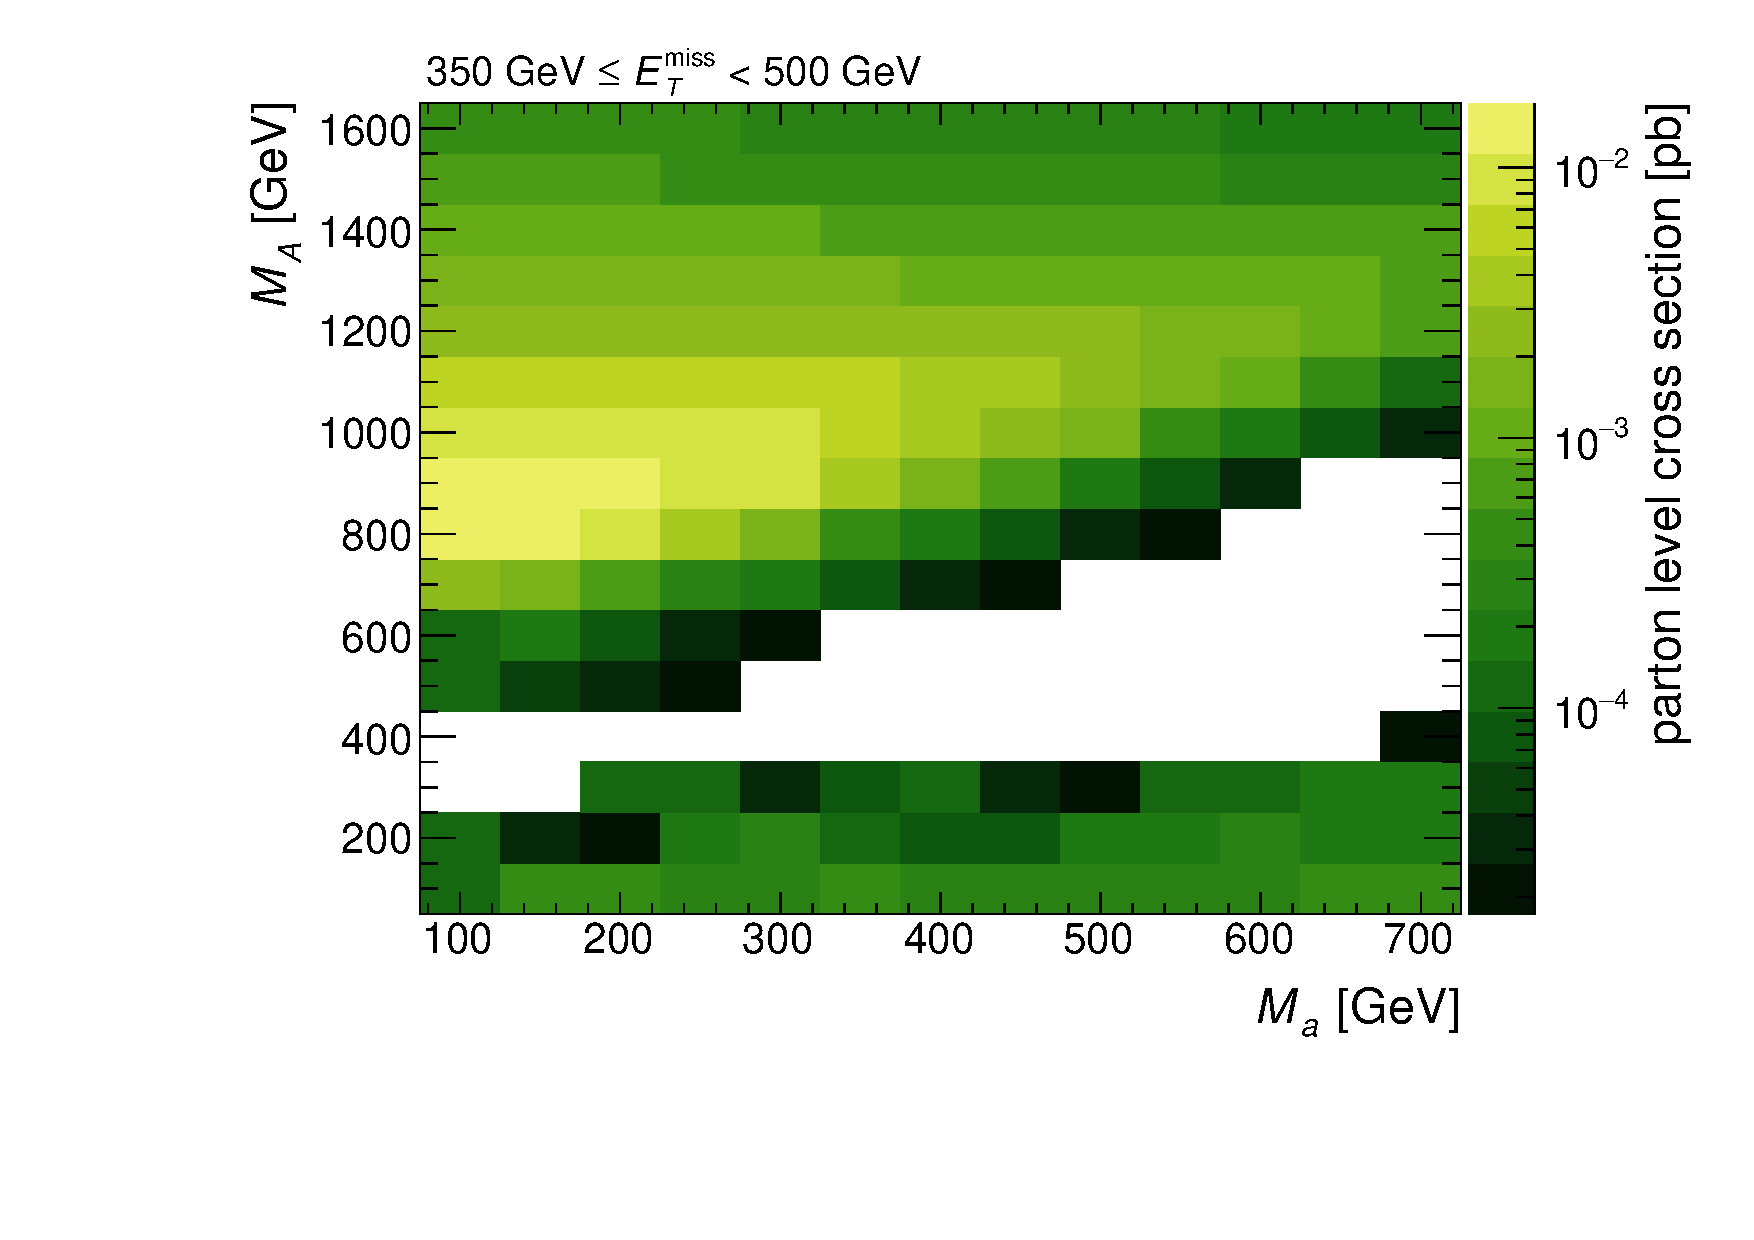
\includegraphics[width = \textwidth]{texinputs/04_grid/figures/monoHbb_parton_level_cross_section_bin_3_ma_vs_mA_lin.pdf}
\end{subfigure}
~
\begin{subfigure}{0.48\textwidth}
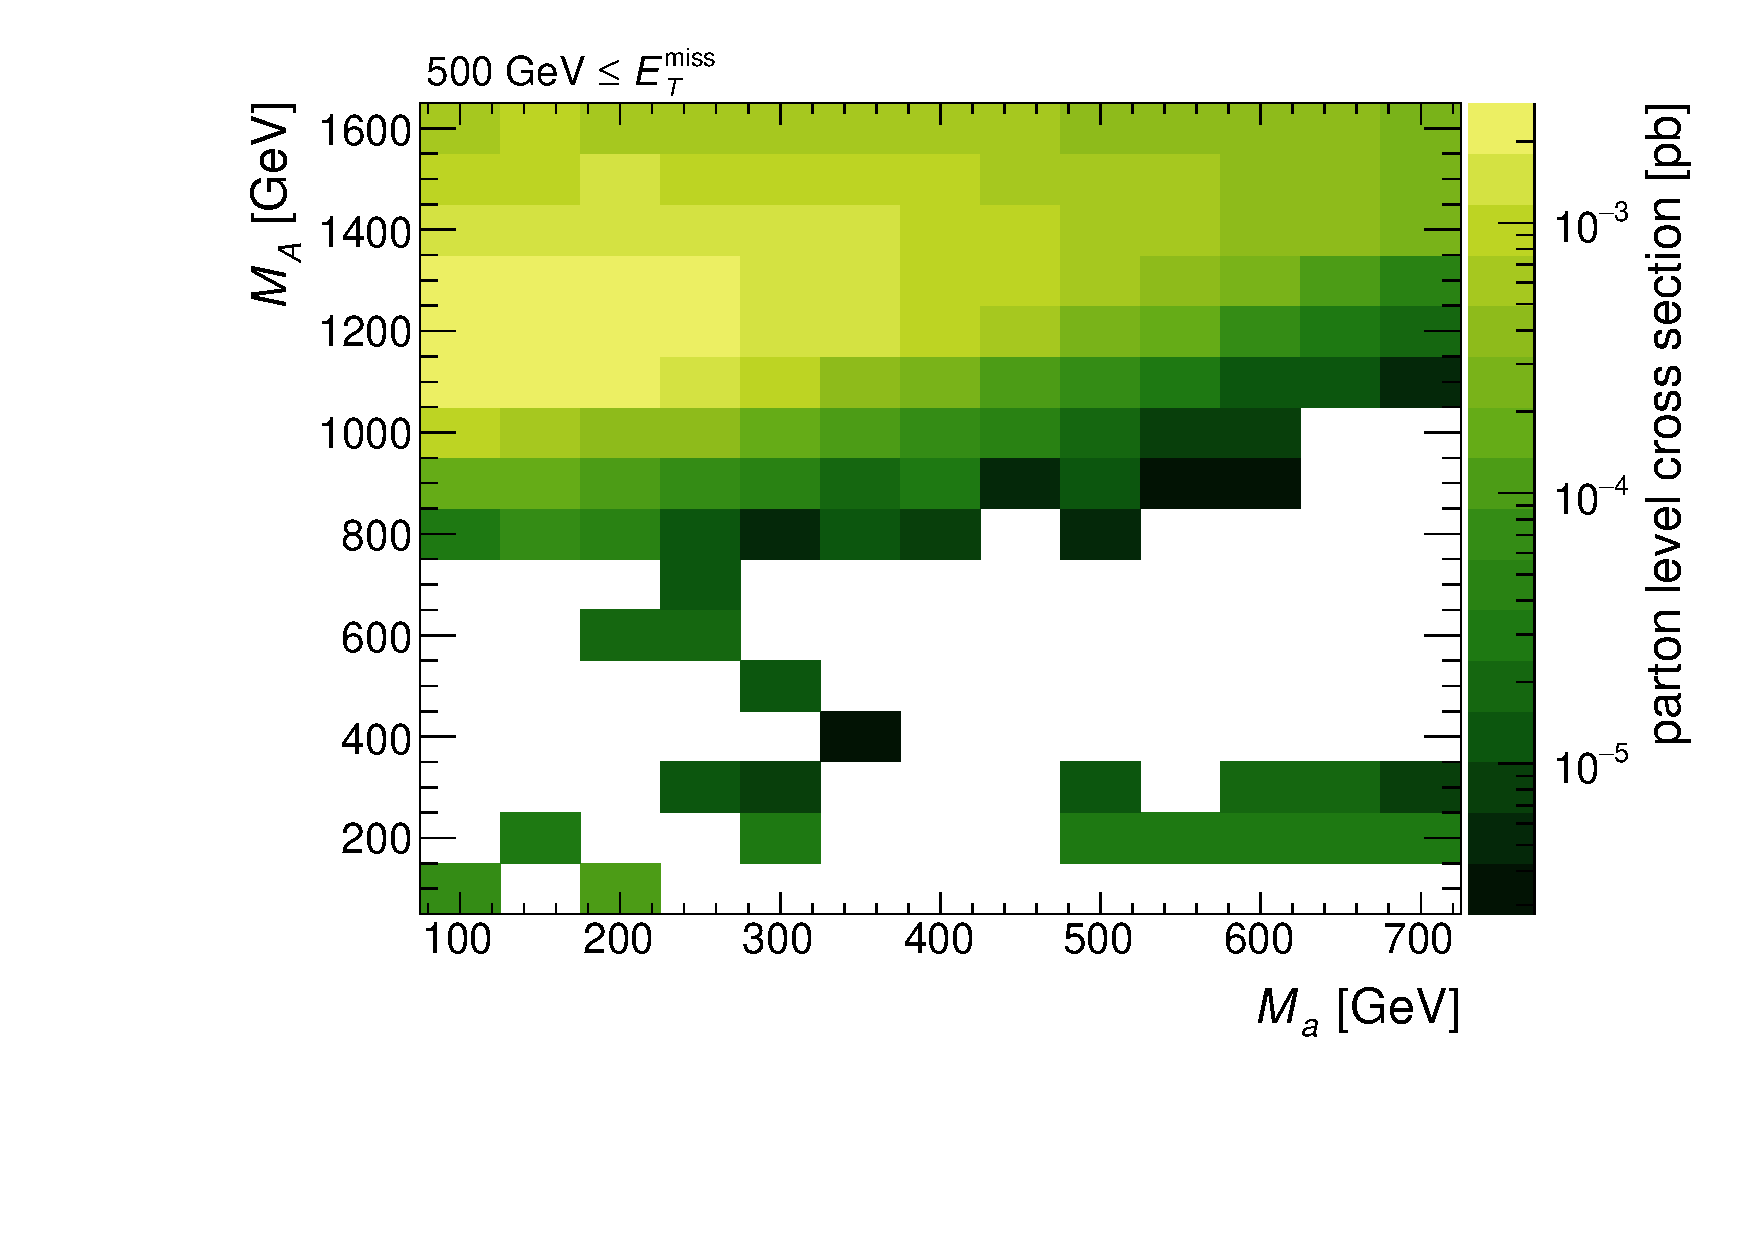
\includegraphics[width = \textwidth]{texinputs/04_grid/figures/monoHbb_parton_level_cross_section_bin_4_ma_vs_mA_lin.pdf}
\end{subfigure}
\caption[$h\to bb + \MET$ cross section binned in $\MET$, $\mA$ - $\ma$ plane ]
{
The production cross section of $h\to bb + \MET$ signal events at parton level as a function of $(\mA,\ma)$ in each of the four \met bins. 
The remaining parameters take the values
$ \mH=\mHc= \mA, \sinp = 0.35, \tanb = 1, \mDM = 10$ GeV and $ \lap1 = \lap2 = \lam3 = 3 $.
}
\label{fig:monoHbb_xsec_bins_mA_ma}
\end{figure}

\begin{figure}[tbp]
\centering
\begin{subfigure}{0.48\textwidth}
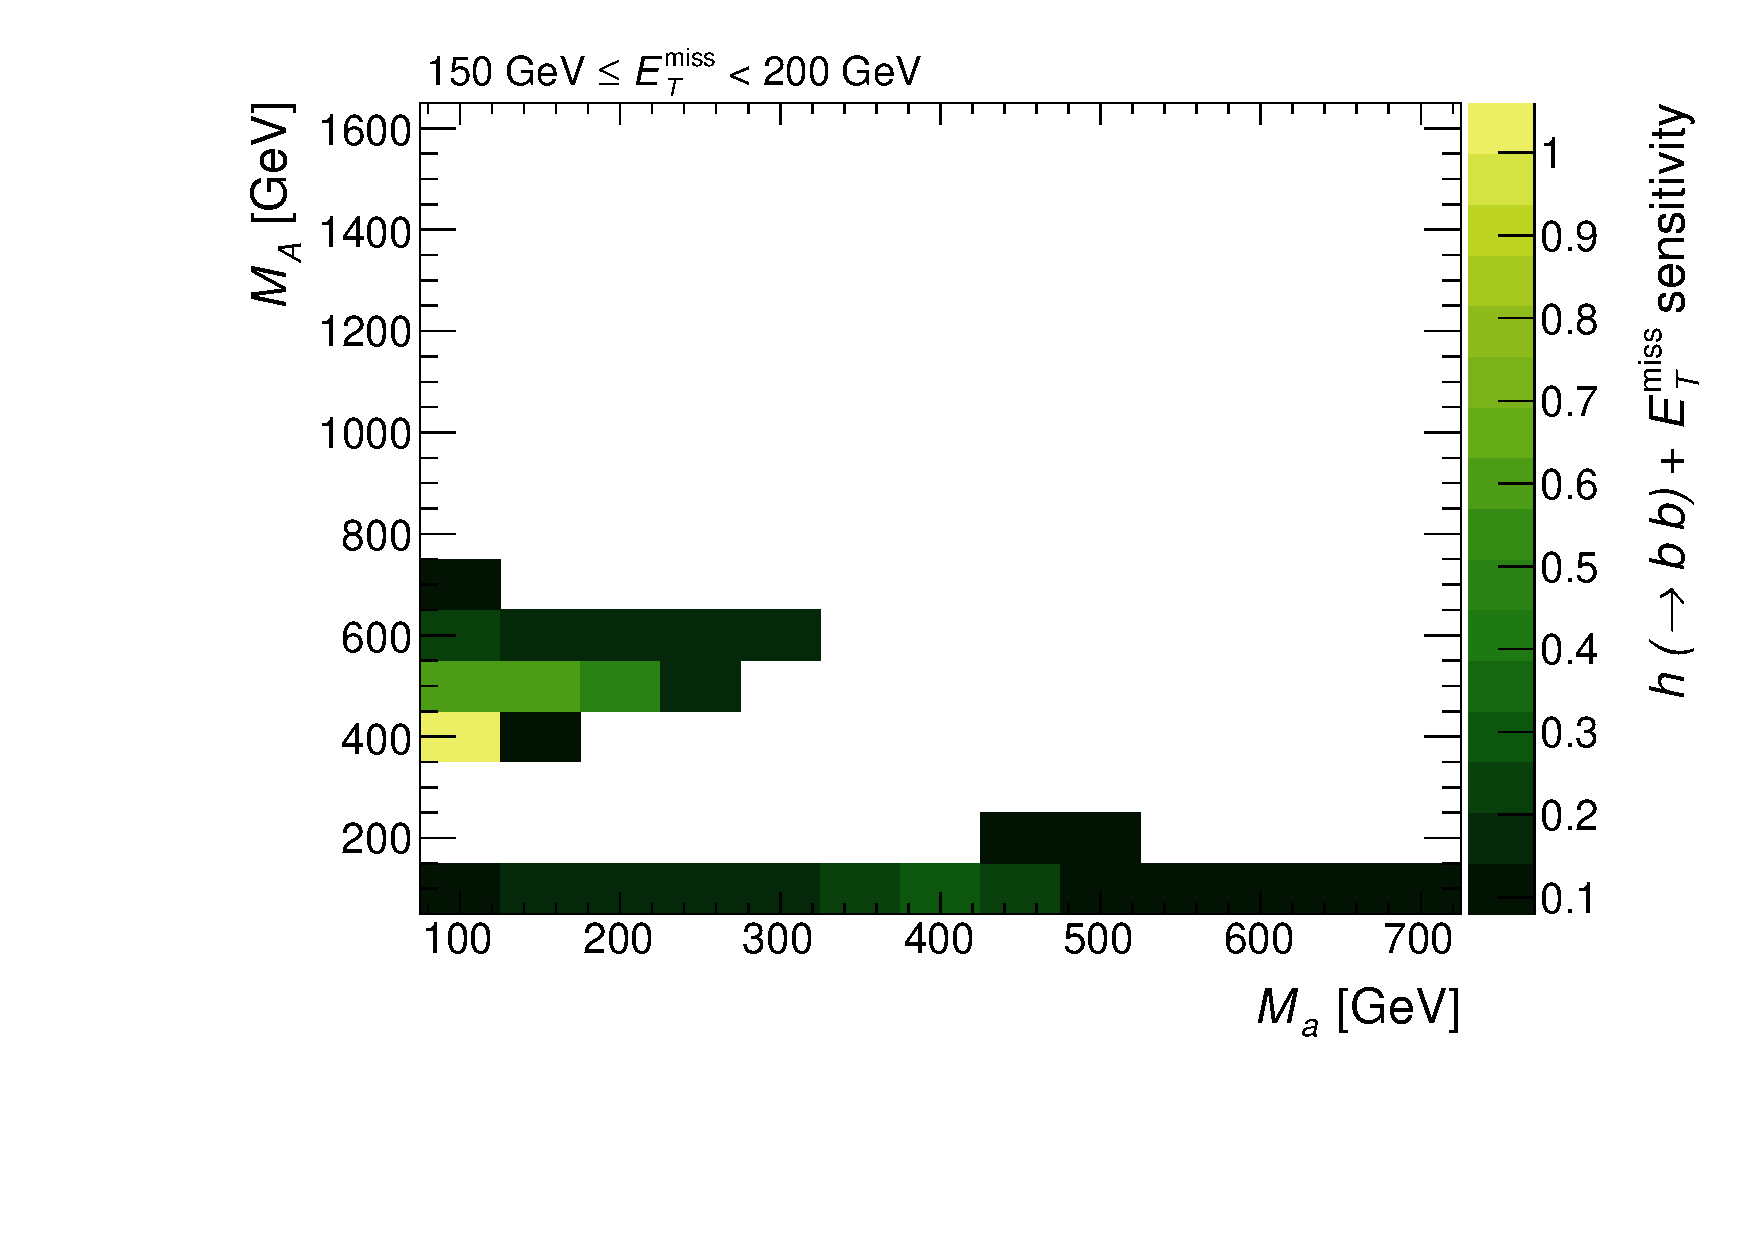
\includegraphics[width = \textwidth]{texinputs/04_grid/figures/monoHbb_sensi_bin_1_ma_vs_mA_lin.pdf}
\end{subfigure}
~
\begin{subfigure}{0.48\textwidth}
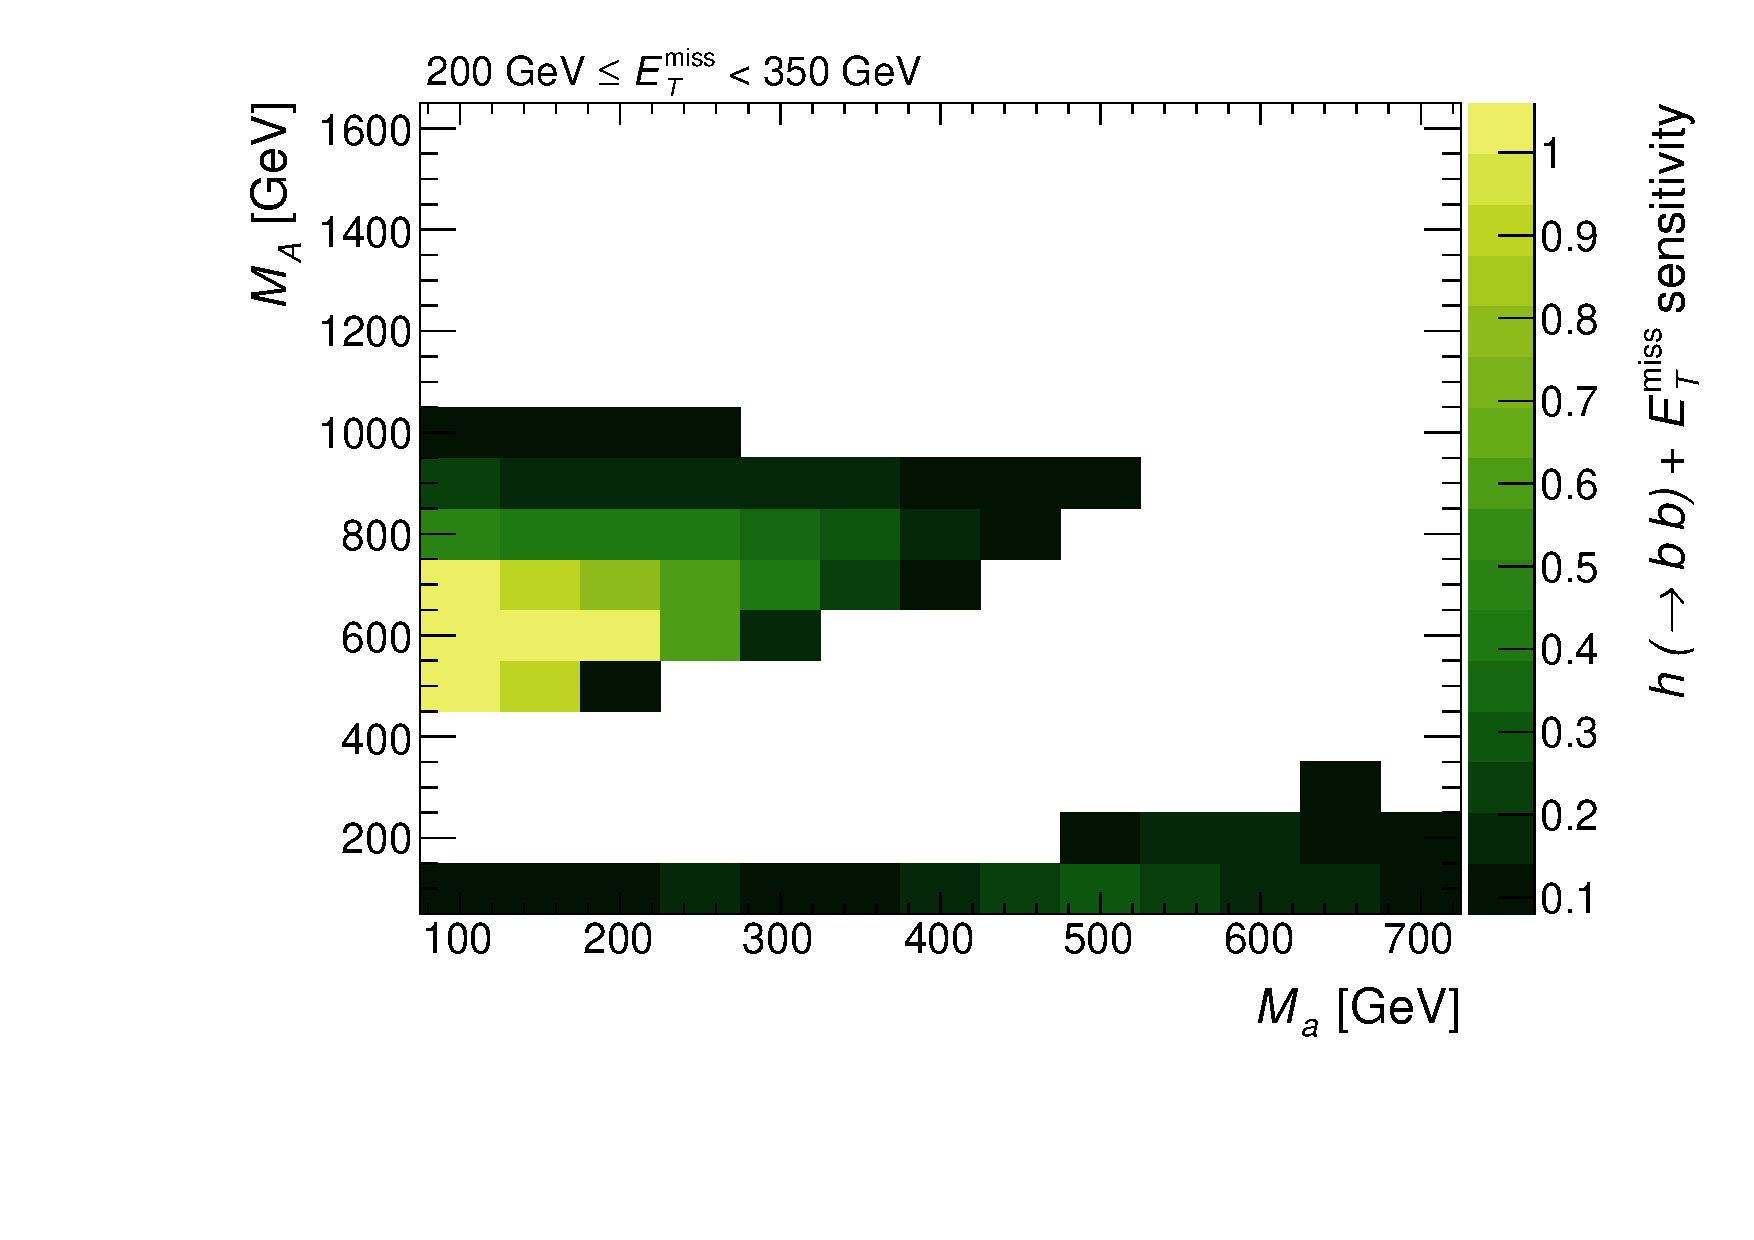
\includegraphics[width = \textwidth]{texinputs/04_grid/figures/monoHbb_sensi_bin_2_ma_vs_mA_lin.pdf}
\end{subfigure}
\\
\centering
\begin{subfigure}{0.48\textwidth}
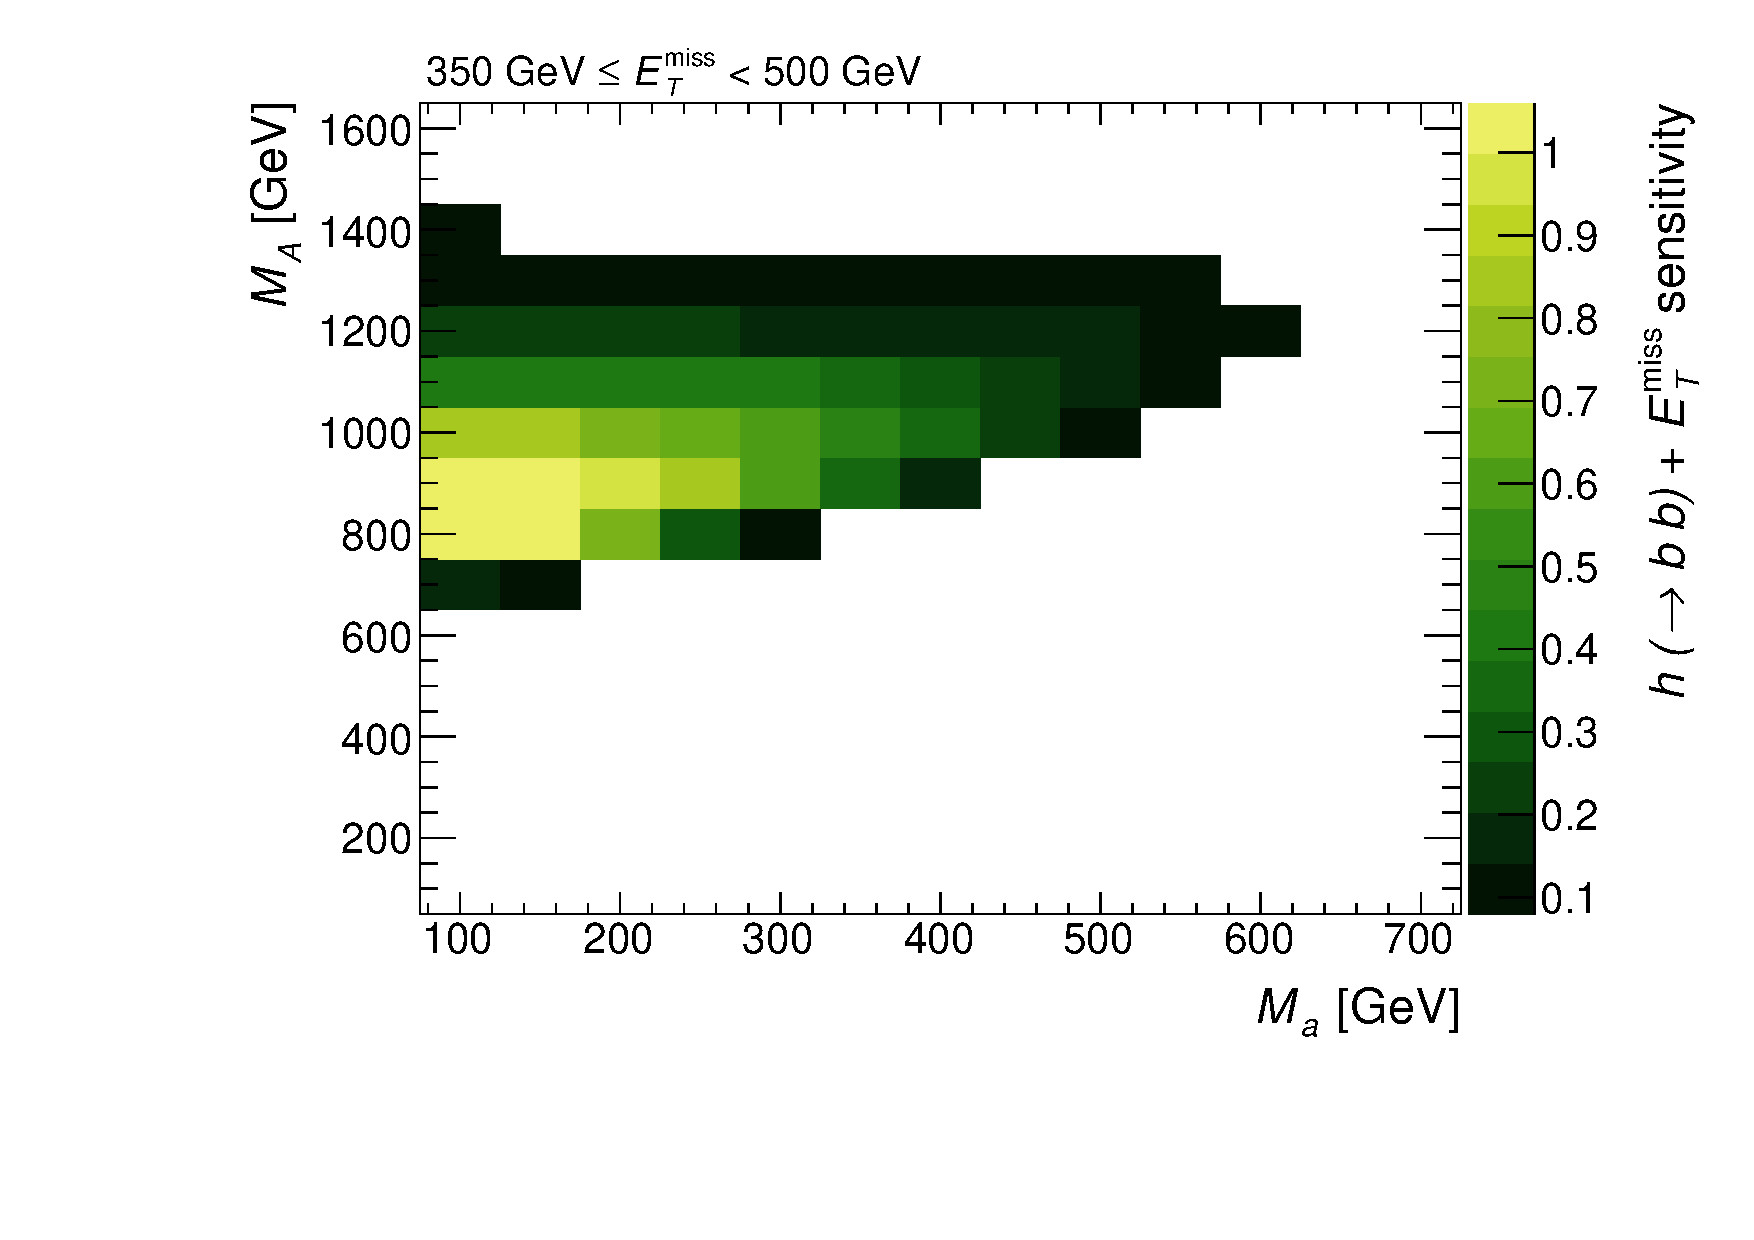
\includegraphics[width = \textwidth]{texinputs/04_grid/figures/monoHbb_sensi_bin_3_ma_vs_mA_lin.pdf}
\end{subfigure}
~
\begin{subfigure}{0.48\textwidth}
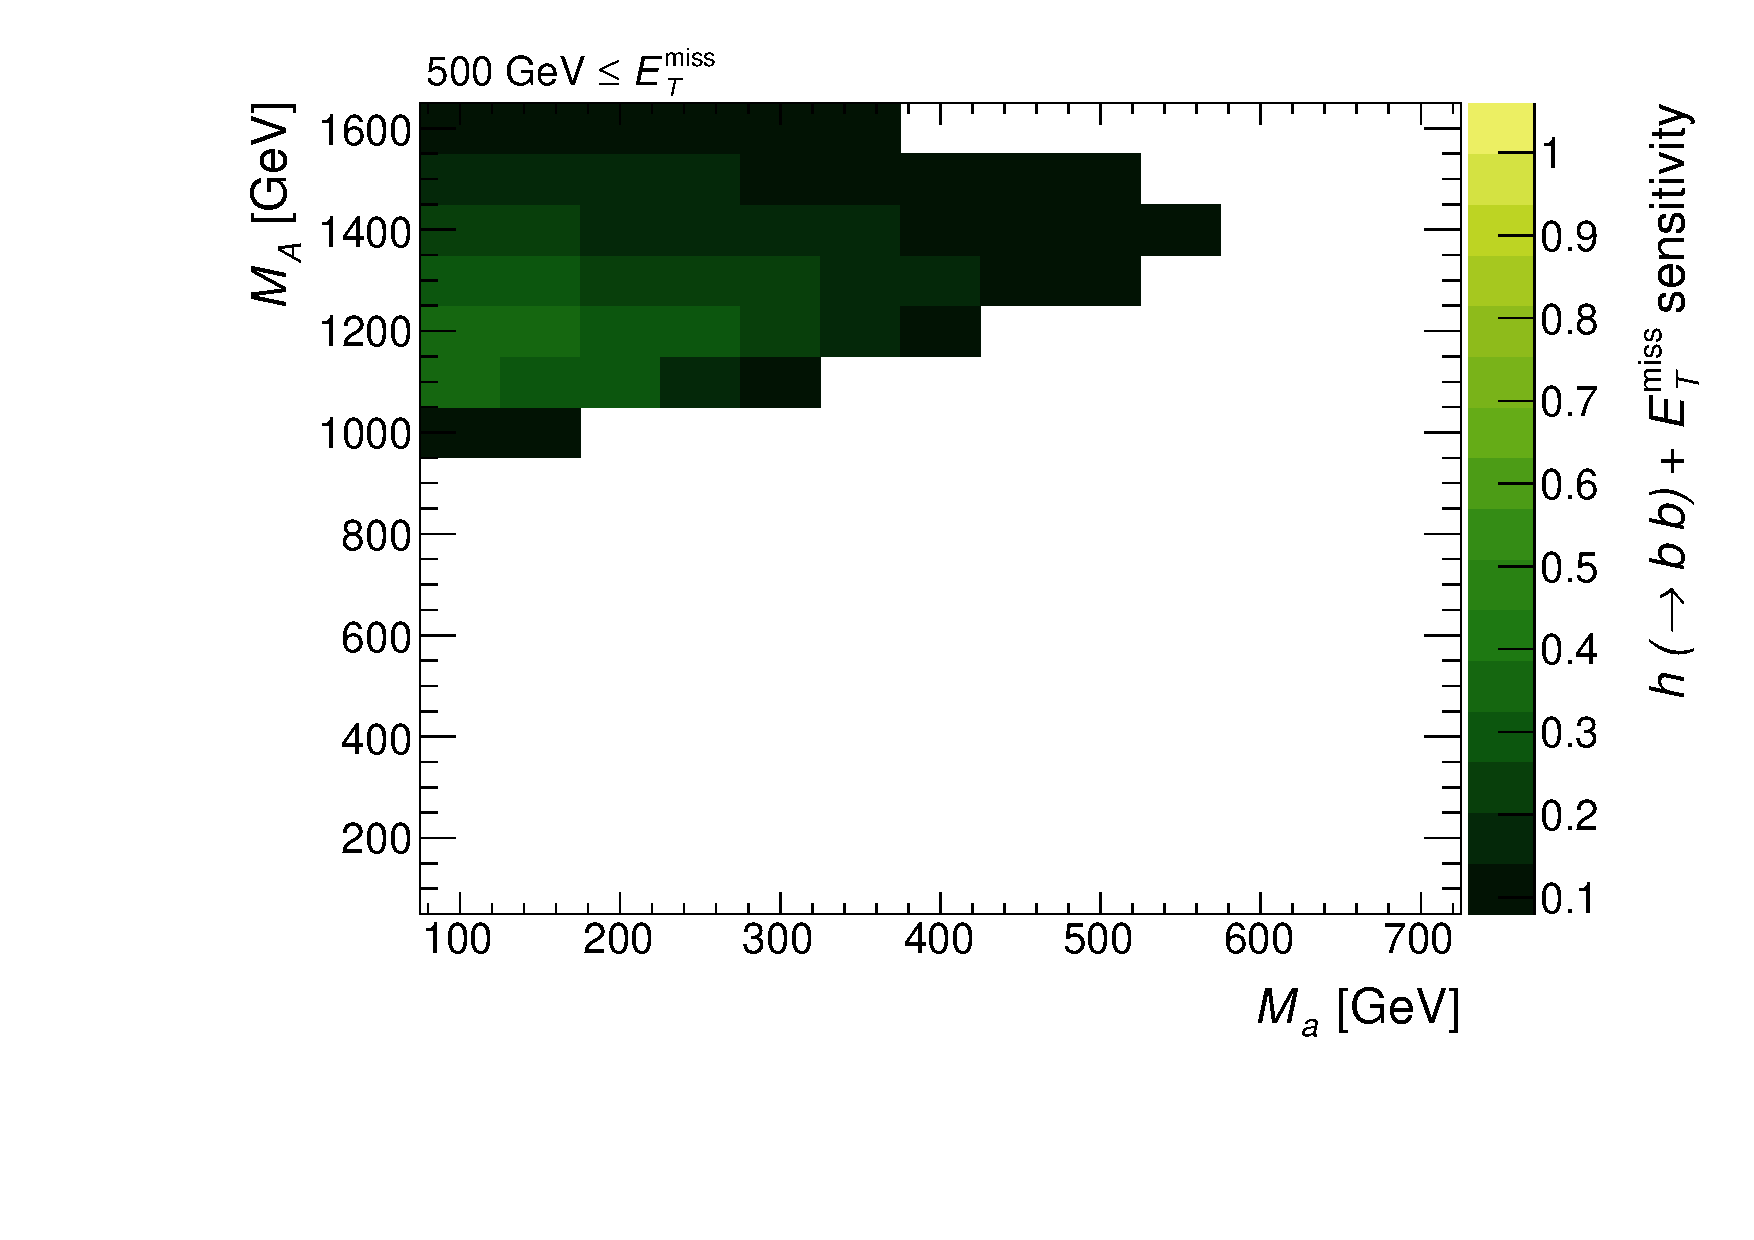
\includegraphics[width = \textwidth]{texinputs/04_grid/figures/monoHbb_sensi_bin_4_ma_vs_mA_lin.pdf}
\end{subfigure}
\caption[Sensitivity to the $h\to bb + \MET$ signal by $\MET$ bin, $\mA$ - $\ma$ plane]
{Estimated sensitivity to $h\to bb + \MET$ events as a function of $(\mA,\ma)$ in each of  the four \met bins. 
The sensitivity, defined in \autoref{eq:monoHbb_sensi}, is based on the limits with reduced model dependence from Ref.~\cite{Aaboud:2017yqz}. 
The remaining parameters take the values
$ \mH=\mHc= \mA, \sinp = 0.35, \tanb = 1, \mDM = 10$ GeV and $ \lap1 = \lap2 = \lam3 = 3 $.}
\label{fig:monoHbb_sensi_bins_mA_ma}
\end{figure}

\begin{figure}[tbp]
\centering
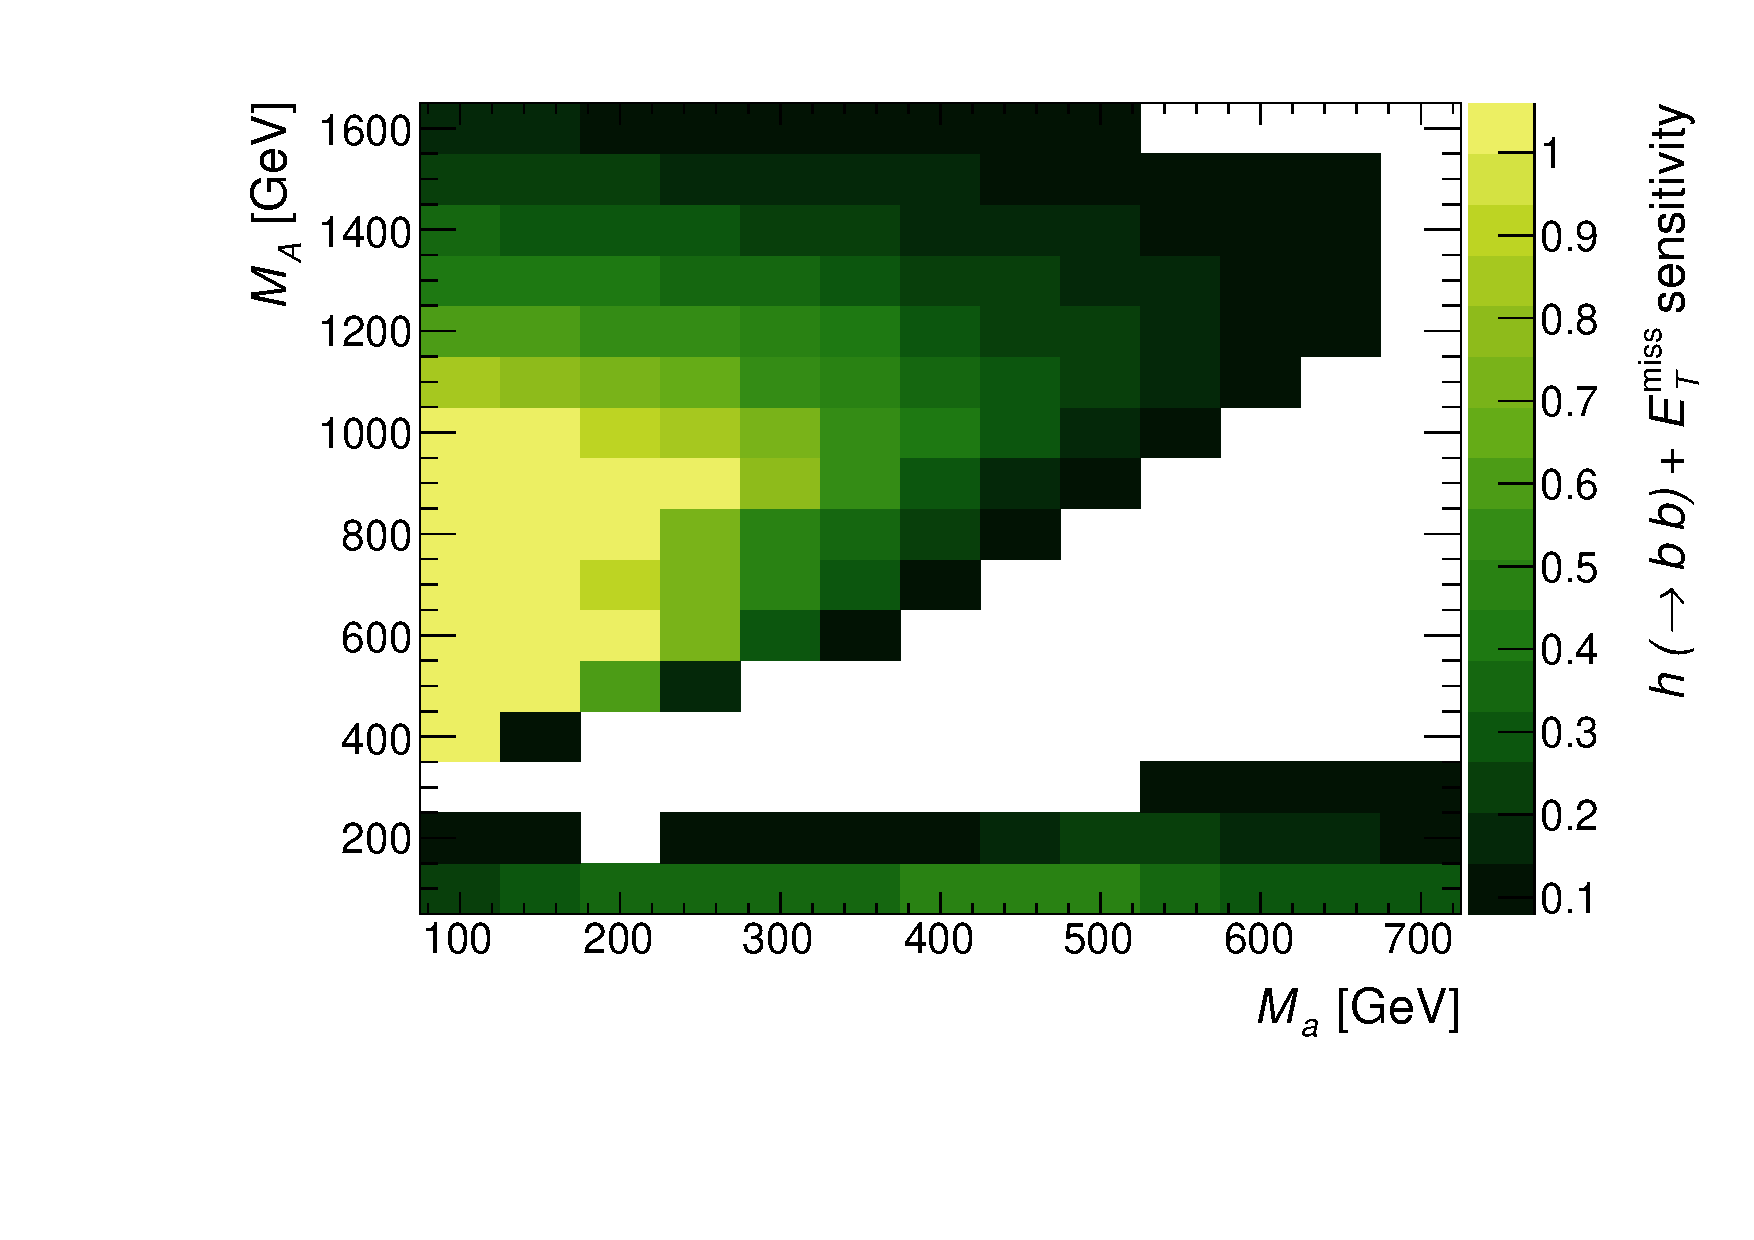
\includegraphics[width=0.7\textwidth]{texinputs/04_grid/figures/monoHbb_sensi_sum_bins_1_2_3_4_ma_vs_mA_lin.pdf}
\caption[Sensitivity to $h\to bb + \MET$ signals in $\mA$ - $\ma$ plane, summed across $\MET$ bins]
{
Sum over all $\MET$-bins of the estimated sensitivity to $h\to bb + \MET$ events as a function of $(\mA,\ma)$. 
The sensitivity, defined in \autoref{eq:monoHbb_sensi}, is based on the limits with reduced model dependence from Ref.~\cite{Aaboud:2017yqz}. 
The remaining parameters take the values $ \mH=\mHc= \mA, \sinp = 0.35, \tanb = 1, \mDM = 10$ GeV and $ \lap1 = \lap2 = \lam3 = 3 $.}
\label{fig:monoHbb_sensi_full_mA_ma}
\end{figure}


\begin{figure}[tbp]
\centering
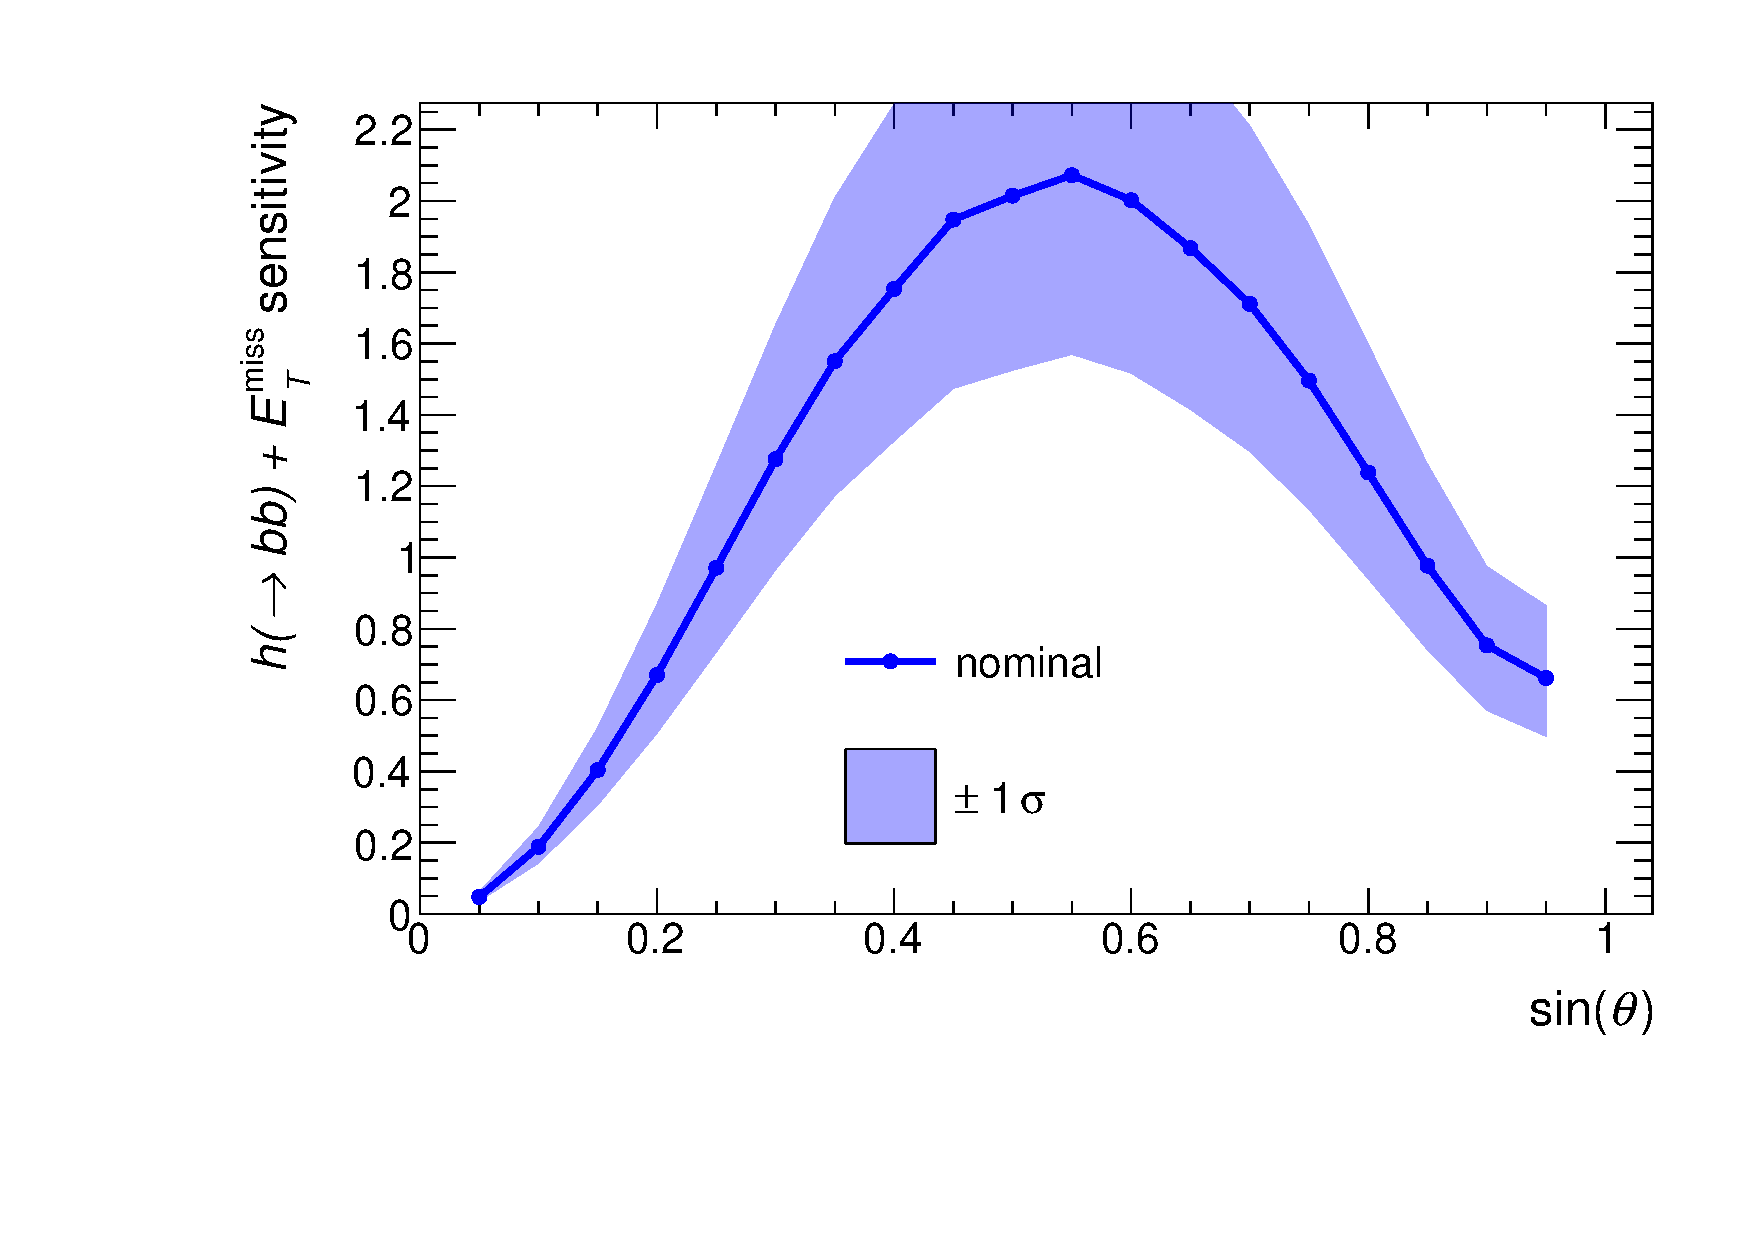
\includegraphics[width=0.49\textwidth]{texinputs/04_grid/figures/monoHbb_sinp_scan_1_sensi_1D.pdf}
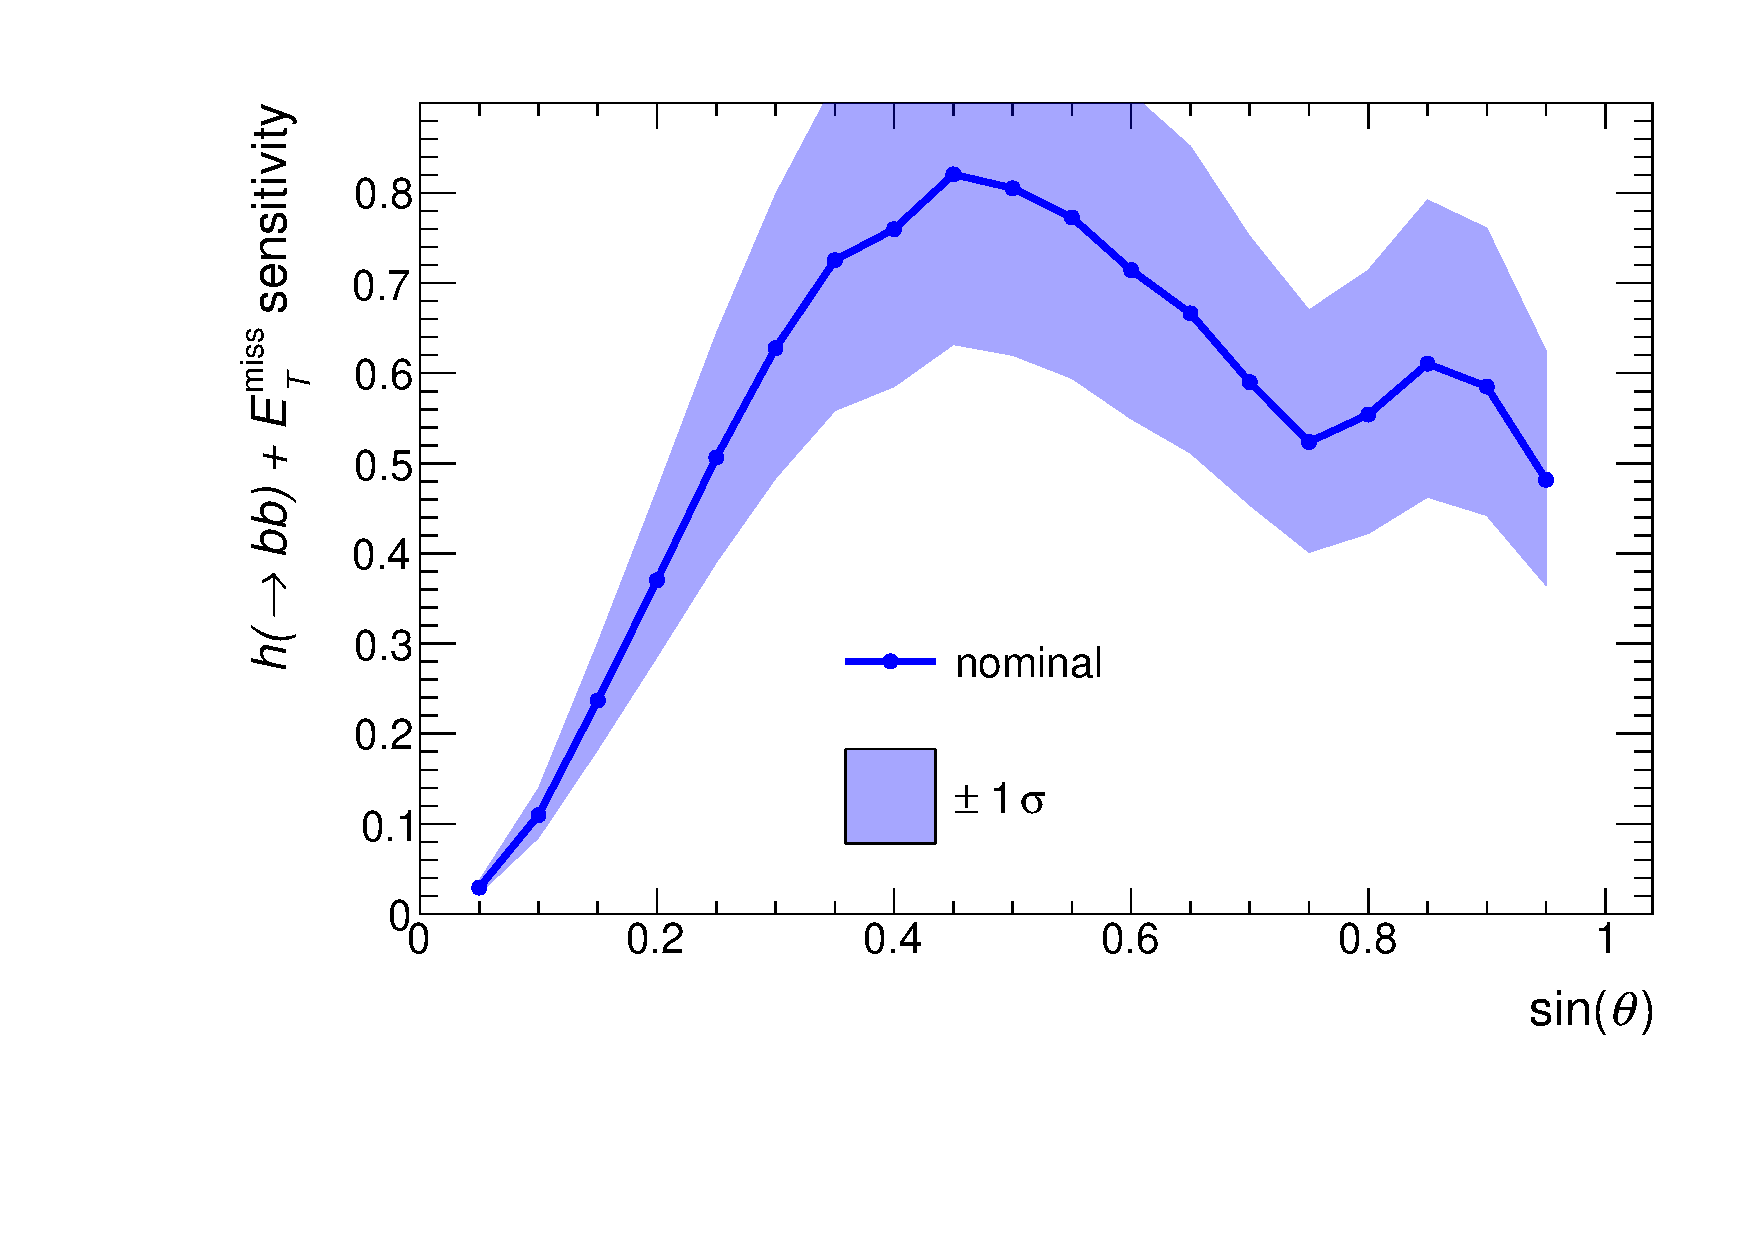
\includegraphics[width=0.49\textwidth]{texinputs/04_grid/figures/monoHbb_sinp_scan_2_sensi_1D.pdf}
\caption[Sensitivity to $h\to bb + \MET$ signals with different $\sinp$, summed across $\MET$ bins]
{
Sum over all $\MET$-bins of the estimated signal sensitivity to $h\to bb + \MET$ events as a function of the pseudoscalar mixing parameter $\sinp$, for $\ma = 200~\GeV$ and $\mH=\mHc=\mA = 600$~GeV~(left) as well as $\ma = 350~\GeV$ and $\mH=\mHc=\mA = 1000$~GeV~(right). The remaining parameters take the values
$\mDM = 10 $ GeV$, \tanb = 1,$ and $ \lap1 = \lap2 = \lam3 = 3 $.
The sensitivity, defined in \autoref{eq:monoHbb_sensi}, as well as the uncertainty on the sensitivity (shaded blue) 
 are based on the limits with reduced model dependence from Ref.~\cite{Aaboud:2017yqz} and the uncertainties described therein. 
}
\label{fig:monoHbb_sensi_full_sinp}
\end{figure}



\begin{figure}[tbp]
\centering
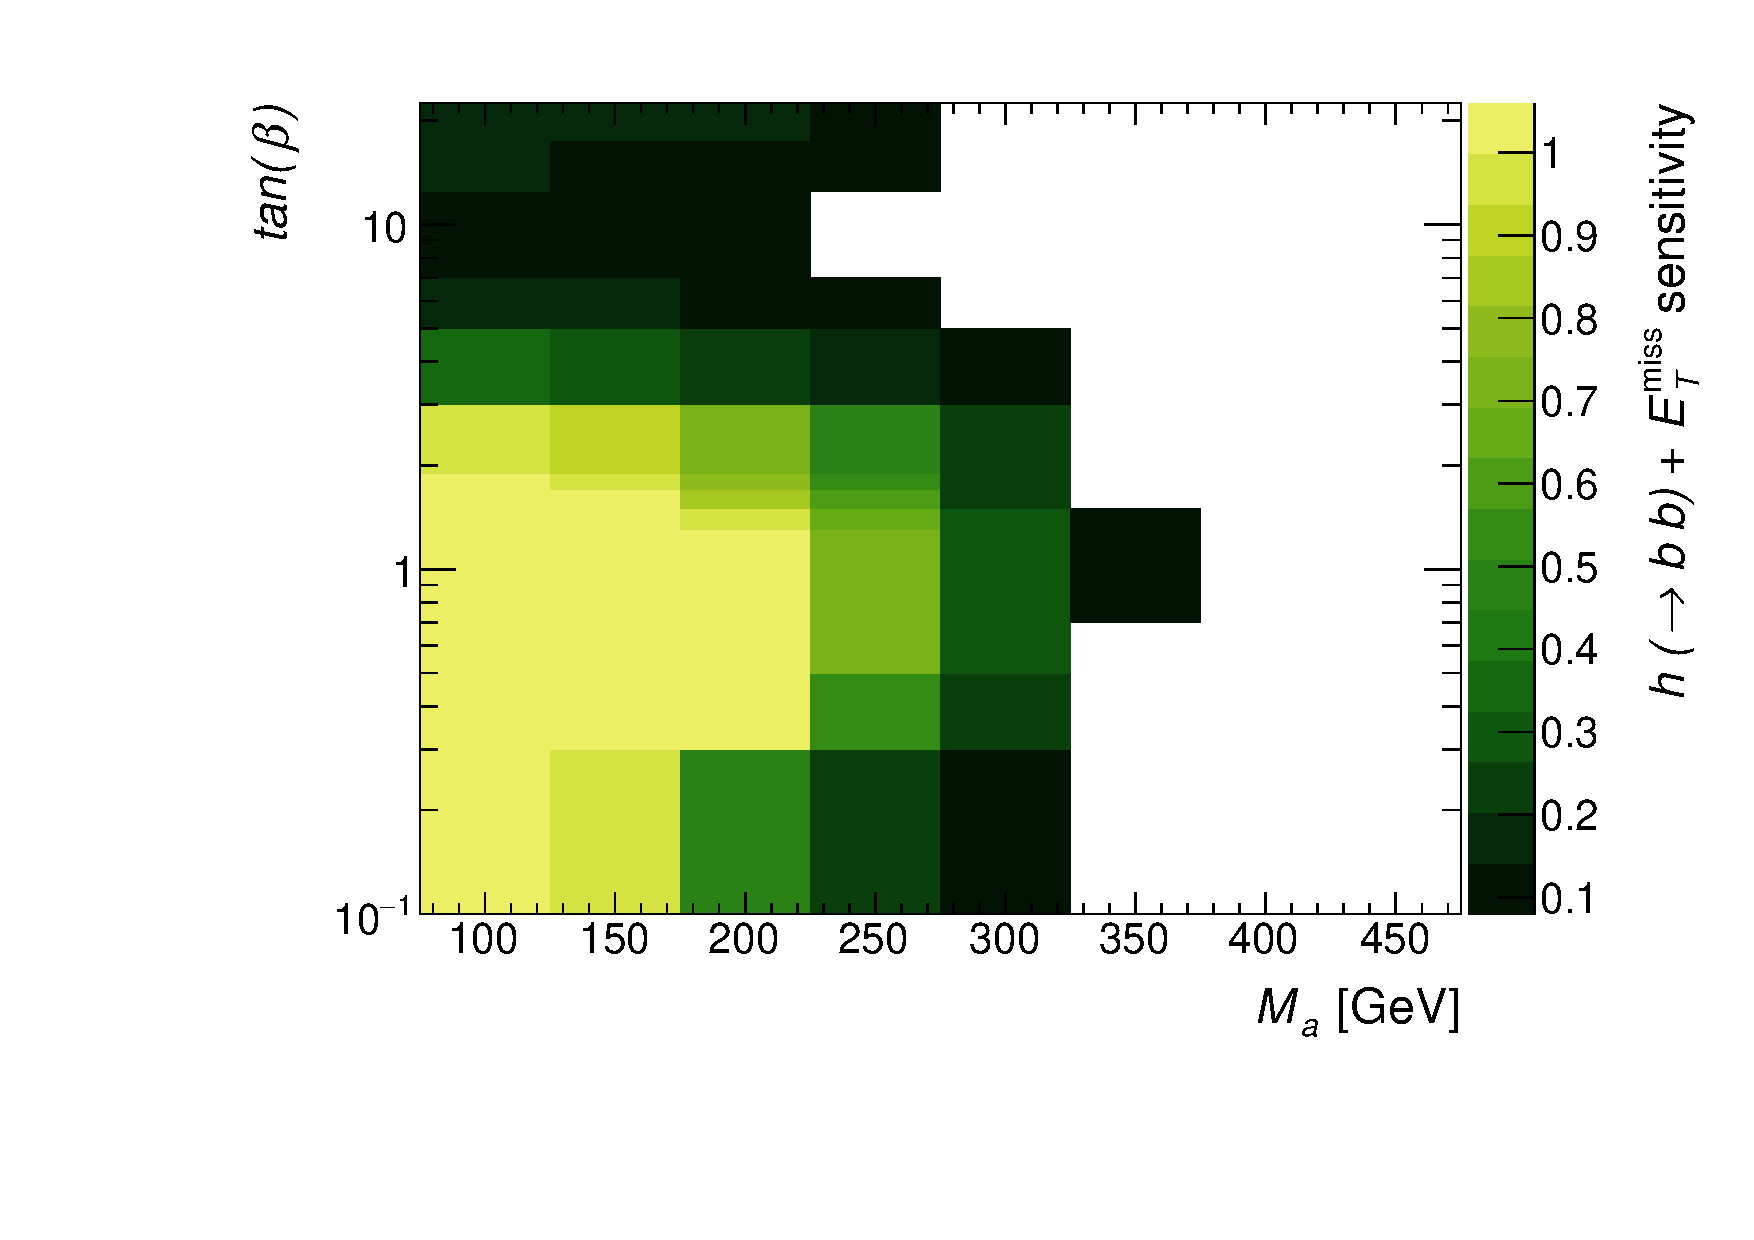
\includegraphics[width=0.7\textwidth]{texinputs/04_grid/figures/monoHbb_sensi_sum_bins_1_2_3_4_ma_vs_tanb_lin.pdf}
\caption[Sensitivity to $h\to bb + \MET$ signals in $\mA$ - $\tanb$ plane, summed across $\MET$ bins]
{
Sum over all $\MET$-bins of the estimated signal sensitivity to $h\to bb + \MET$ events as a function of $(\ma,\tanb)$. The sensitivity, defined in \autoref{eq:monoHbb_sensi}, is based on the limits with reduced model dependence from Ref.~\cite{Aaboud:2017yqz}. The remaining parameters take the values
$ \mH=\mHc=\mA = 600$ GeV, $ \sinp = 0.35, \mDM = 10$ GeV and $ \lap1 = \lap2 = \lam3 = 3 $.}
\label{fig:monoHbb_sensi_full_ma_tanb}
\end{figure}

\begin{figure}[tbp]
\centering
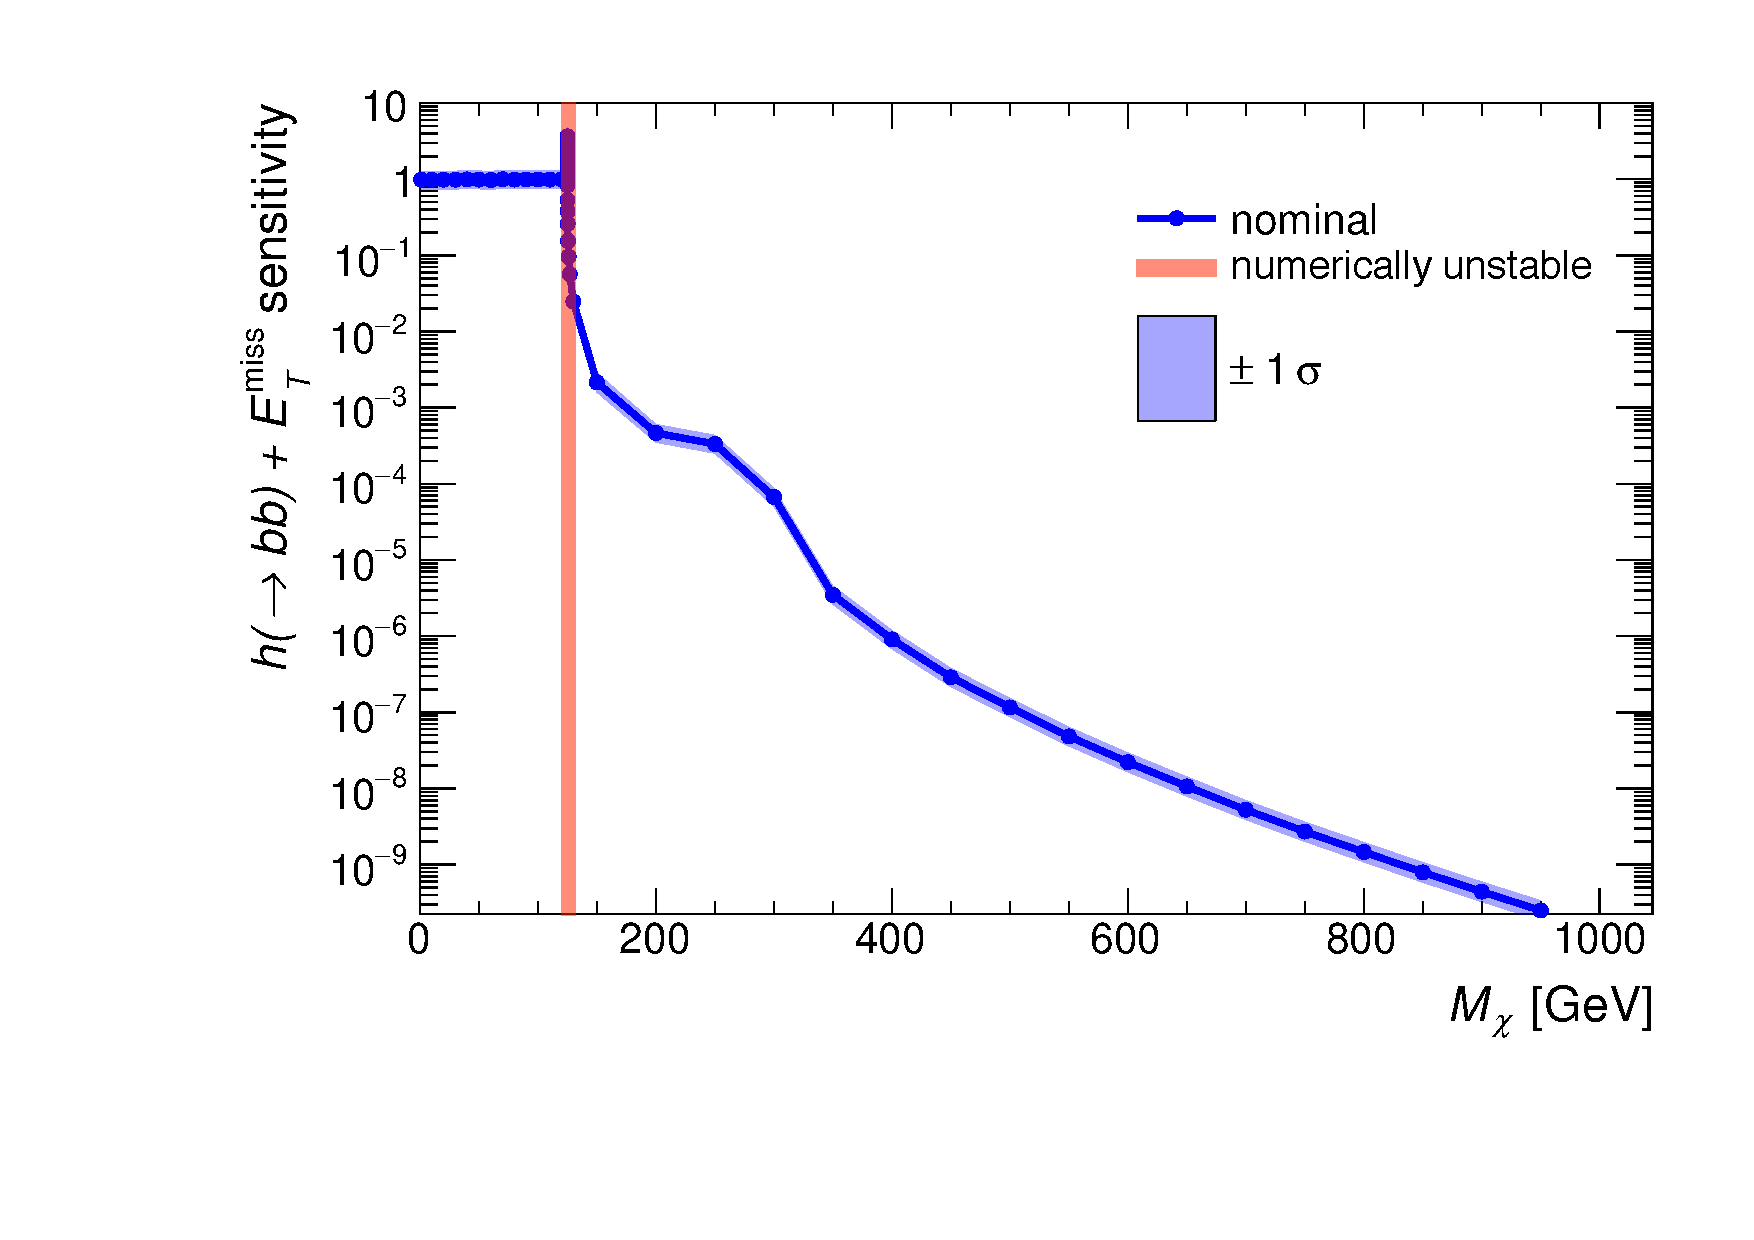
\includegraphics[width=0.7\textwidth]{texinputs/04_grid/figures/monoHbb_sensi_mDM_scan.pdf}
\caption[Sensitivity to $h\to bb + \MET$ signals with different $\mDM$, summed across $\MET$ bins]
{
Sum over all $\MET$-bins of the estimated signal sensitivity to $h\to bb + \MET$ events as a function of the DM mass $\mDM$. 
The sensitivity, defined in \autoref{eq:monoHbb_sensi}, as well as the uncertainty on the sensitivity (shaded blue)
are based on the limits with reduced model dependence from Ref.~\cite{Aaboud:2017yqz} and the uncertainties described therein. 
The remaining parameters take the values
$ \ma = 250 $ GeV$, \mH=\mHc=\mA = 600$ GeV, $ \sinp = 0.35, \tanb = 1,$ and $ \lap1 = \lap2 = \lam3 = 3 $. 
The sensitivity is constant below $\mDM < \ma/2$, and rapidly drops for $\mDM > \ma/2$. The sensitivity is resonantly enhanced for $\mDM = \ma/2$.}
\label{fig:monoHbb_sensi_full_mDM}
\end{figure}

The sensitivity estimate of ATLAS and CMS to the \hdma scenario through the \monohbb signature is based on limits on anomalous production of 125 GeV Higgs bosons in association with \met with minimal model dependence~\cite{Aaboud:2017yqz}. The limits are translated to parton level and compared to parton-level simulations of the \hdma scenario for the sensitivity estimate. This approach avoids the simulation of the detector response, which requires a significant amount of computing resources, and more iterations and refinements of the signal grid can be performed. 

The limits with minimal model dependence are provided in terms of the detector-level cross section of $\monohbb$ events $\sigma_{i}^{\mathrm{obs},\,\monohbb}$ as a function of \met in four bins $i=1,...4$~\cite{Aaboud:2017yqz}. 
To compare these values to the simulation results at parton level, 
an estimate of the detection efficiency $\varepsilon$ times the kinematic acceptance $\mathcal{A}$ of the event selections of the analysis is used for each of the four $\MET$ bins.
%This estimate is provided as one $(\mathcal{A\times\varepsilon})$ value for each of the four $\MET$ bins. 
Thus, the $(\mathcal{A}\times\varepsilon)_i$ figure represents the minimum probability
that an event generated at parton level in a given $\MET$ bin $i$ is reconstructed in that same $\MET$ bin and passes all analysis selections.
%The limits with minimal model dependence are provided separately for each of the four $\MET$ bins used in \cite{Aaboud:2017yqz}.
%Thus, the simulated evebts are binned into those bins (\autoref{fig:monoHbb_xsec_bins_mA_ma}).
Consequently, the cross section for \hdm production in the \hdma scenario at parton level $\sigma_{i}^{\mathrm{parton},\,\hdm}$ is calculated in the same $\MET$ bins as used in the \monohbb search. This starting point is shown in \autoref{fig:monoHbb_xsec_bins_mA_ma} using the scan in $(\mA,\ma)$ as a representative example. 
In the next step, the sensitivity $\sens_i$ for each of the \met bins $i=1,...4$ is calculated as
\begin{equation}
\label{eq:monoHbb_sensi_i}
\sens_i \equiv \frac{\sigma_{i}^{\mathrm{parton},\,\hdm} \times \mathcal{B}^{\mathrm{SM},\,h\to bb} \times (\mathcal{A\times\varepsilon})_{i} }
{\sigma_{i}^{\mathrm{obs},\,\monohbb}}\,,
\end{equation}
where $\mathcal{B}^{\mathrm{SM},\,h\to bb}$ is the $h\to bb$ branching ratio predicted by the SM for the 125~GeV Higgs boson. A representative example for this step is given in \autoref{fig:monoHbb_sensi_bins_mA_ma} for the scan in $(\mA,\ma)$.  A particular point in the $(\mA,\ma)$ parameter parameter space is excluded if $\sens_i \geq 1$. Finally, to obtain a single estimate for the total sensitivity $\senstot$ using all four $\MET$ bins, their individual contributions from \autoref{eq:monoHbb_sensi_i} are summed over\footnote{
This choice is made because the individual per-bin sensitivities follow a logarithmic metric, and because a model will typically populate several \met bins at a time. This implies that there could be models where $\sens_i<1$ in every bin, yet the sum from \autoref{eq:monoHbb_sensi} is $>1$.
Therefore, for a rigorous exclusion of a model based on the limits with minimal model dependence, the preferred approach would be to consider only the most sensitive bin for the exclusion.
}:
\begin{equation}
\label{eq:monoHbb_sensi}
\senstot \equiv \sum_{i\in\met~\mathrm{bins}} \sens_i\,.
\end{equation}
The resulting $\senstot$ is shown in \autoref{fig:monoHbb_sensi_full_mA_ma} for the example of the $(\mA,\ma)$ scan.


The scan of the sensitivity in the sense of \autoref{eq:monoHbb_sensi} in the $(\ma,\mA)$ plane is shown in \autoref{fig:monoHbb_sensi_full_mA_ma}.
The sensitivity decreases with increasing $\mA = \mH = \mHc$ for $\mA \geq 1$~TeV because the fraction of resonant signal events drops. 
This drop is caused by increasingly large $\Gamma_A$, 
which allows for an increasing fraction of non-resonant signal events, driven by events with very off-shell $A$. % ref ggF-> A -> ah feynman graph
%Non-resonant signal events have soft $\MET$ and thus the search is less sensitive to them, since the minimum accepted $\MET$ is $\MET \geq 150$ GeV.
Near the mass diagonal $\ma = \mA$, there is little to no sensitivity. 
This is because the Jacobian peak moves to low $\MET$ for a small mass splitting $|\mA - \ma|$
(\autoref{eq:monoH_peak_met}, \autoref{fig:monoHbb_mA_scan_met}, and \autoref{fig:monoHbb_ma_scan_met}).
Beyond this, the coupling $g_{Aah}$ is small when all Higgs bosons are nearly degenerate in mass, cf.~Equation~4.12 in Ref.~\cite{Bauer:2017ota}, %ref to eq.in theory part(?)
resulting in a small total cross section and therefore further decrease in sensitivity.
The sensitivity above the mass diagonal, $\mA > \ma$, is larger than below the mass diagonal.
Two parameter choices cause this asymmetry:
\begin{enumerate}
\item 
$\mA = \mH = \mHc$, i.e., the neutral and charged $CP$-even scalars have low masses below the diagonal, but high masses above it, introducing an asymmetry.
Another effect can be seen in \autoref{fig:monoHbb_mH_scan_met}: values of  $\mH = \mHc$ below the mass of the higher-mass pseudoscalar (in this case $A$)
give a reduced total cross section and a lower fraction of resonant signal events. Both effects reduce sensitivity;
\item 
$\sinp = 0.35 \neq 1/\sqrt{2}$, i.e. the mixing between the pseudoscalars $A$ and $a$ is asymmetric. 
$A$ couples more strongly to SM particles than $a$, and vice versa for the couplings to the DM fermion $\chi$.
So the situation below the diagonal corresponds to the case of $\sinp = \sqrt{1-0.35^2} \approx 0.938$ and $\mA > \ma$. 
As can be seen in \autoref{fig:monoHbb_sinp_scan_mA600_ma200_met},
this \sinp configuration has a higher fraction of non-resonant signal events with low \met, and correspondingly a lower sensitivity is found in \autoref{fig:monoHbb_sensi_full_sinp}.
\end{enumerate}

The scan of the sensitivity in the  $(\ma,\tanb)$ plane is shown in  \autoref{fig:monoHbb_sensi_full_ma_tanb}. 
At very low $\tanb$, the Yukawa coupling to top quarks is large, and most of the signal events come from non-resonant processes, as can be seen from \autoref{fig:monoHbb_tanb_scan_met}. % ref to tanb met scan
The non-resonant processes are characterised by soft $\MET$, which lowers the kinematic acceptance and reduces the sensitivity of the search.
For higher $\tanb$, the fraction of resonant events increases due to the reduced top Yukawa coupling, resulting in an increase of sensitivity.
However, reducing the top Yukawa coupling also reduces the total production cross section. 
This effect is sub-dominant below $\tanb \approx 1.2$, and the sensitivity increases with $\tanb$. 
But above $\tanb \approx 1.2$, the sensitivity loss due to reduced cross section outpaces the sensitivity gain due to a more resonant signal.
Overall, the search gets less sensitive with increasing $\tanb$ above $\tanb \approx 1.2$.
At very high $\tanb$ ($\geq 10$), this trend is reversed again because the $\tanb$ enhancement\footnote{The \hdma scenario assumes a Yukawa sector of type II.} of the 
coupling to $b$-quarks compensates for the small $b$-quark mass.
At this point $bb$ initiated processes start to dominate the production cross section and drive the increase in sensitivity.

The sensitivity to models with varying $\sinp$ is shown in \autoref{fig:monoHbb_sensi_full_sinp}.
The sensitivity vanishes at $\sinp=0$ and $\sinp=1$, since those values correspond to no mixing between $A$ and $a$, and thus no connection between the SM and the dark sector. 
For its intermediate values, the $\sinp$ parameter influences the couplings of the pseudoscalars to DM as well as to SM fermions, 
and also the coupling strength of trilinear scalar vertices such as $g_{Aah}$~\cite{Bauer:2017ota}. 
Increasing the couplings increases the total cross section. 
However, increasing some couplings can also increase $\Gamma_A$ and thereby decrease the resonant fraction of signal events and the sensitivity.
The upshot of this is that there can be more than one local maximum in the sensitivity curve, as shown the right panel of~\autoref{fig:monoHbb_sensi_full_sinp}. 
The precise dependence of the sensitivity on \sinp depends on the precise interplay of the couplings.
Because the couplings depend on all other model parameters including all the Higgs masses, 
tuning the $\sinp$ of a parameter scan to the sensitivity in a single point can lead to sub-optimal sensitivity in other points.

The sensitivity to models with varying $\mDM$ is shown in  \autoref{fig:monoHbb_sensi_full_mDM}.
Below the threshold of $\mDM < \ma/2$, the sensitivity is constant since the $\MET$ distribution and the total signal cross section remain invariant, as demonstrated in \autoref{fig:monoHbb_mDM_scan_met}.
At threshold, the sensitivity is enhanced because the partial width for $ a \to \chi \chi $ is enhanced, 
increasing the signal cross section.
Above threshold, the sensitivity drops rapidly because $\mDM > \ma/2$ requires an off-shell $a^{\star} \to \chi\chi$ decay, which is strongly suppressed by the typically  narrow width of $a$. 
The width of $a$ is substantially reduced once $a\to \chi \chi$ is kinematically inaccessible, 
as $\Gamma_{a\to \chi \chi}$ is a large contribution to the total width of $a$ for $\mDM \leq \ma/2$ \cite{Bauer:2017ota}.
There is a slight increase in sensitivity for $\mDM \approx \mA/2$ when the $A\to \chi\chi$ decay hits its kinematic threshold, yet the absolute sensitivity remains negligible.
